%%%%%%%%%%%%%%%%%%%%%%%%%%%%%%%%%%%%%%%%%%%%%%%%%%%%%%%%%%%%%%%%%%%%%%%%%%%%%%%%%%%%%%%%%%%%%%%
%                                          HYPEROPT                                           %
%%%%%%%%%%%%%%%%%%%%%%%%%%%%%%%%%%%%%%%%%%%%%%%%%%%%%%%%%%%%%%%%%%%%%%%%%%%%%%%%%%%%%%%%%%%%%%%
\chapter{Hyper-parameter Optimization of Neural Networks}
\label{chap:hyperopt}

\begin{chapabstract}
This chapter introduces the problem of hyper-parameter optimization for neural networks, which is the problem of automatically finding the optimal architecture and training setting for a particular task. Section~\ref{sec:ho_lit} presents the problem and the existing approaches while Section~\ref{sec:bo} explains in depth the method of Bayesian optimization which is used for the rest of the chapter. A performance improvement of this method is given in Section~\ref{sec:cholesky}. In Section~\ref{sec:compare}, we compare the performance of random search and Bayesian optimization on a toy problem and give theoretical bounds on the performance of random search. We propose a new method in Section~\ref{sec:cap}, which combines Bayesian optimization with another method, Hyperband. Finally, we apply Bayesian optimization to the practical problem of MRI field-of-view classification in Section~\ref{sec:isbi}.
\end{chapabstract}

\vspace{1cm}

{   
    \setstretch{1.0}
    \minitoc
}

\newpage

%%%%%%%%%%%%%%%%%%%%%%%%%%%%%%%%%%%%%%%%%%%%%%%%%%%%%%%%%%%%%%%%%%%%%%%%%%%%%%%%%%%%%%%%%%%%%%%
\section{Defining the Problem}
\label{sec:ho_lit}

The problem of hyper-parameter optimization appears when a model is governed by hyper-parameters, i.e. parameters that are not learned by the model but must be chosen by the user. Automated methods for tuning them become worthwhile when hyper-parameters are numerous and difficult to manually tune due to a lack of understanding of their effects. The problem gets worse when the hyper-parameters are not independent and it becomes necessary to tune them at the same time. The most intuitive solution is to test all possible combinations by discretizing the hyper-parameter space and choosing an order of evaluation, a method called \textit{grid search}. This method does not scale because the number of combinations grows exponentially with the number of hyper-parameters, making this approach usually unusable for neural networks.

In practice, as it is usually impossible to prove the optimality of a solution without testing all solutions, the accepted solution is the best found in the budget allocated by the user to the search.

Even though this problem appears in all kinds of situations, we are interested here in the optimization of deep learning models, as they have many hyper-parameters and we lack the understanding and the theoretical tools to tune them. The hyper-parameters fall in two categories: the ones that affect the architecture of the network (such as the number or type of layers) and the ones that affect the training of the network (such as the learning rate or the batch size).

In the case of deep learning, evaluating a combination (a specific network) is costly in time and computing resources. Moreover we have little understanding of the influence of each hyper-parameter on the performance of the model, resulting in very large boundaries and a much bigger space than needed. The situation is even worse since combinations near the boundaries of the hyper-parameter space can build a network too big to fit in the available memory, requiring to have a way to handle evaluation failures. 

While it is tempting to simply return an extremely bad performance, this causes problems to methods assuming some structure in the hyper-parameter space. For example, a continuous hyper-parameter that gives a smooth output will suddenly have a discontinuity, and a method assuming smoothness (such as Bayesian optimization) might not work anymore. In practice, there are method-dependent solutions to this problem. 

%%%%%%%%%%%%%%%%%%%%%%%%%%%%%%%%%%
\subsection{Notations}
\label{ssec:notation}

In this chapter we refer to a \textit{model} as a neural network, even though the black-box methods presented in Section~\ref{ssec:black_box} work for other machine learning models. The \textit{parameters} of a model are the weights of the network which are learned during training. The \textit{hyper-parameters} are the parameters governing the architecture of the networks (such as the number of layers or the type of layers) and the ones governing the training phase (such as the learning rate or the batch size). 

A \textit{hyper-parameter space} $\mathrm{X}$ is a hypercube where each dimension is a hyper-parameter and the boundaries of the hypercube are the boundaries of each hyper-parameter. Each point in the hyper-parameter space is referred to as a \textit{combination} $\mathrm{x} \in \mathrm{X}$. To each combination is associated a value $\mathrm{y}$ corresponding to the performance metric of the underlying neural network on the task it is trained to solve. We name $f$ a function taking as input a combination $\mathrm{x}$, build and train the underlying model and output its performance $f\left( \mathrm{x} \right)$.

Concretely in the case of deep learning, $f$ is the process that build and train a neural network specified by a set of hyper-parameters $\mathrm{x}$, and returns the loss of the model which serves as the performance metric.

%%%%%%%%%%%%%%%%%%%%%%%%%%%%%%%%%%
\subsection{Black-box optimization}
\label{ssec:black_box}

From the notation of Section~\ref{ssec:notation}, the goal of hyper-parameter optimization is to find the combination $\mathrm{x_*}$ minimizing the performance $\mathrm{y}$ (typically the performance is a loss function, which we want to minimize):
\begin{equation}
	\mathrm{x_*} = \argmin_{\mathrm{x} \in \mathrm{X}} f(\mathrm{x})
\end{equation}

This is the problem of hyper-parameter optimization viewed as black-box optimization. Methods in this category are independent from the model and could be used for any kind of mathematical function. However the hyper-parameters we are interested in are of a varied nature (continuous, discrete, categorical), limiting us to derivative-free optimization methods. This section is not a complete review of derivative-free algorithms, but an overview of the popular algorithms used specifically for hyper-parameter optimization.

\subsubsection{Grid search}

The most basic method is usually called \textit{grid search}. Very easy to implement, it simply tests every possible combination (typically with uniform sampling for the continuous hyper-parameters). With only a handful of hyper-parameters to optimize and with a function $f$ fast to evaluate, it can be advisable to use as a first step to get sensible boundaries on each hyper-parameter, i.e. by testing a handful of values over a very wide range to find a smaller but relevant range.

But in the context of deep learning, hyper-parameters are too numerous, meaning there are too many combinations to evaluate, and each evaluation is costly. Limiting oneself when choosing the hyper-parameters still leaves us with at least 5 or 6 hyper-parameters but it is easy to end up with over 30 hyper-parameters. Assuming an average of 4 values per hyper-parameters, this implies $4^5 = 1024$ combinations for a space of 5 hyper-parameters or $4^{30} \simeq 10^{18}$ combinations with 30 hyper-parameters. Grid search does not scale well, which makes it unsuitable for deep learning.

Even for reasonably sized hyper-parameter space, a typical implementation in nested for-loops goes from one corner of the hyper-parameter space to the opposite corner in fixed order. It is unlikely that the corner the search starts from happens to be an area filled with good models, since combinations in corners are extreme values of hyper-parameters and build atypical neural networks. 

Grid search can still be used with a wide enough sampling of the hyper-parameters to get an idea on where the interesting models are located and refine the boundaries, but even for that other methods are preferable.

\subsubsection{Random search}

One step above grid search is \textit{random search}. A big limitation of grid search is that the order it goes through the hyper-parameter space is very dependent on the implementation and it always selects the same limited set of values for each hyper-parameter. Random search instead draws the value of each hyper-parameter from a uniform distribution, allowing for a much wider range of explored values.

\begin{figure}[htb]
	\begin{minipage}[b]{.49\linewidth}
		\centering
		\centerline{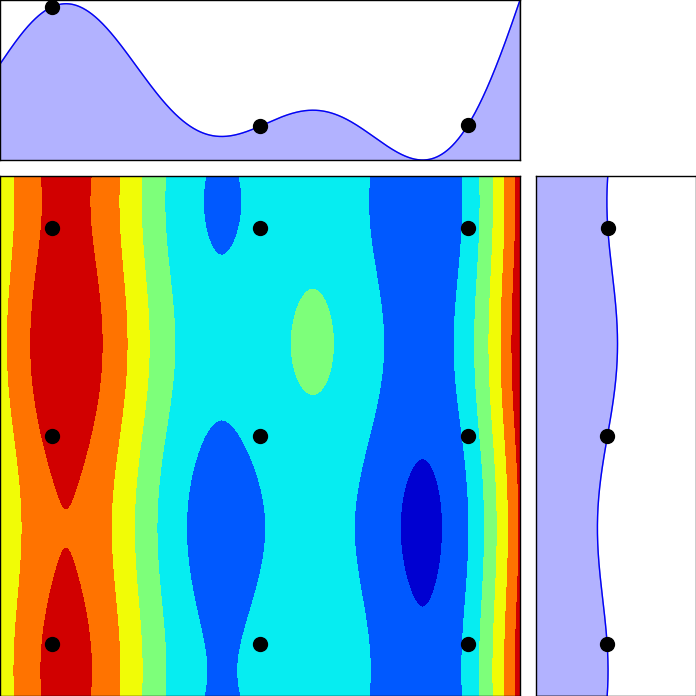
\includegraphics[width=7.2cm]{img_hyperopt/rs_grid}}
	\end{minipage}
	\begin{minipage}[b]{.49\linewidth}
		\centering
		\centerline{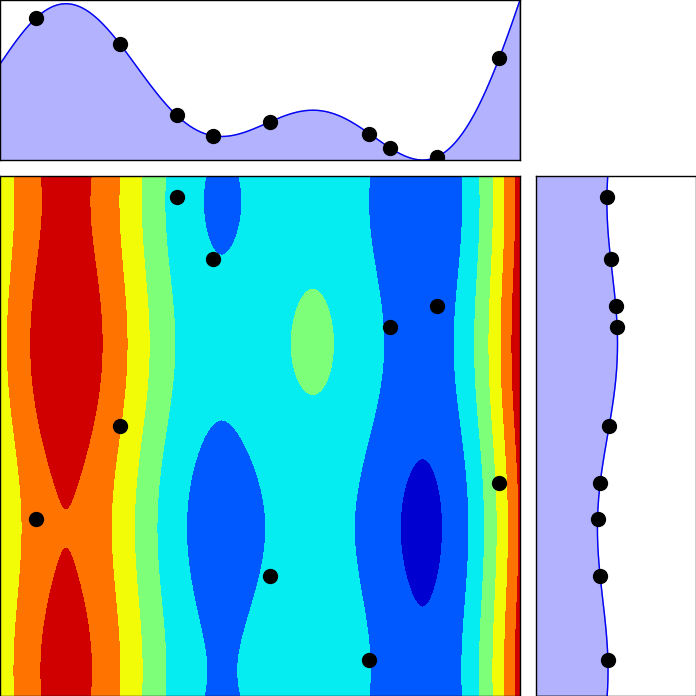
\includegraphics[width=7.2cm]{img_hyperopt/rs_random}}
	\end{minipage}
	\caption[Comparison of grid search and random search]{Loss function for a two dimensional space. (Left) Grid search. (Right) Random search. 9 combinations were tested for each method, but grid search tested only 3 values for each hyper-parameters while random search tested 9, resulting in a better solution.}
	\label{fig:rs}
\end{figure}

Figure~\ref{fig:rs} illustrates this. Given a hyper-parameter space of two continuous hyper-parameters, and at equal number of evaluated combinations, random search finds a better solution. It works because hyper-parameters are not equally relevant. In practice, for deep learning, only a few have a high impact on the performance (\textcite{bergstra2012JMLR}).\footnote{We do not know in advance which hyper-parameters have a high impact, otherwise we would tune only high impact hyper-parameters.} In the figure, grid search only tested three values of each hyper-parameters while random search tested nine for the same cost!

In terms of implementation cost, random search requires only the ability to draw uniformly from an interval or a list, giving it the same computational cost than grid search. The increased implementation cost is largely compensated by the gain in performance.

\subsubsection{Bayesian optimization}

Going further requires some assumption about the structure of the hyper-parameter space. Namely, similar values for an hyper-parameter results in similar performance, i.e. some weak notion of continuity. If there is some structure, we can exploit it.

Bayesian optimization (\textcite{bergstra2011NIPS}), which we present in details in Section~\ref{sec:bo}, applies this idea by modeling $f$ with as few evaluations as possible while searching for the best combination. It comes with a non-trivial implementation cost, though packages are available. In Section~\ref{sec:compare} we compare the performance of random search and Bayesian optimization on a practical task.

%%%%%%%%%%%%%%%%%%%%%%%%%%%%%%%%%%
\subsection{Evolutionary algorithms}

The first application of evolutionary algorithms to neural networks was to evolve the weights of a fixed architecture (\textcite{miller1989}). A few years later,~\textcite{braun1993} and~\textcite{angeline1994} realized it was more efficient to evolve simultaneously the weights and the topology of the network. Further refinements of these approaches led to the \textit{NeuroEvolution of Augmenting Topologies} (NEAT) algorithm (\textcite{stanley2002EC}). 

NEAT uses three kinds of mutations (modifying a weight, adding a connection between two nodes and adding a node in the middle of a connection) and one kind of recombination based on fitness sharing. Many variants of this algorithm have been proposed, notably HyperNEAT (\textcite{stanley2009}) which only evolves the topology and learns the weights by back-propagation. 

The main drawback of NEAT and its variants is their inability to scale and evolve the large networks typical of modern deep learning.~\textcite{real2017ICML} and~\textcite{miikkulainen2017} developed approaches able to explore extremely diverse and atypical network structures and find architectures with state-of-the-art performance on computer vision tasks such as CIFAR-10. 

The drawback of those methods however is their excessive computational cost, requiring thousands of iterations before starting to build good models. Coupled with their novelty, those methods were out of our reach, while the lack of scaling was too important in the older methods for us to use them in this thesis. 

%%%%%%%%%%%%%%%%%%%%%%%%%%%%%%%%%%
\subsection{Reinforcement learning}

Recent advances in reinforcement learning have made possible its use to design efficient neural networks. The idea is to train an agent called the controller which builds neural networks for a specific task.~\textcite{baker2017ICLR} developed a controller that chooses each layer of the network sequentially and is trained using Q-learning.~\textcite{zoph2017ICLR} created a string representation of neural networks and their controller is a RNN outputting valid strings. In both cases the created networks must be fully trained to be evaluated and the controller takes thousands of iterations to converge, making those approaches extremely costly.

To address this problem,~\textcite{zoph2017} proposed testing on a smaller dataset as an approximation of the performance on the true dataset. Another suggestion is to train only partially each network (\textcite{li2017ICLR},~\textcite{zela2018}), allowing longer training time as the search is refined.

While those approaches are very promising, they are too recent and costly for this thesis.

%%%%%%%%%%%%%%%%%%%%%%%%%%%%%%%%%%
\subsection{Other approaches}

We finish our tour with a few methods taking radically different approaches. Hyperband (\textcite{li2017ICLR}) considers the question as a multi-armed bandit problem, where each arm is a combination and we have a finite amount of training budget to allocate to each arm. The idea is to train many models partially, and take the decision to continue training every few epochs based on the current performance. Since we chose to explore this approach, we present it in more details in Section~\ref{ssec:hyperband}.

\textcite{hazan2018ICLR} proposed an approach applying compressed sensing to hyper-parameters optimization called Harmonica. Like Bayesian optimization, they aim to learn the structure of the hyper-parameter space, but using a sparse polynomial.

Finally,~\textcite{domhan2015} suggested predicting the learning curve of a model to decide whether to continue the training. The prediction is done using a portfolio of parametric models.

%%%%%%%%%%%%%%%%%%%%%%%%%%%%%%%%%%
\subsection{Synthesis}
\label{ssec:synthesis}

\begin{sidewaystable}[htbp]
	\centering
	\begin{tabular}{ | l | c | c | c | c | c | c | c | c | c | }
		 \rota{} & \rota{Grid Search} & \rota{Random Search} & \rota{Bayesian Optimization - GP} & \rota{Bayesian Optimization - Tree} & \rota{Evolutionary Algorithms} & \rota{Reinforcement Learning} & \rota{Extrapolation of Learning Curves} & \rota{Hyperband} & \rota{Harmonica} \\ 
		\hline
		Black-box? & \checkmark & \checkmark & \checkmark & \checkmark & & & & & \checkmark \\
		Does not require structure in $\mathrm{X}$? & \checkmark & \checkmark & & & & & & \checkmark & \\
		Conditional hyper-parameters? & & & & \checkmark & \checkmark & \checkmark & & & \\
		Training method hyper-parameters? & \checkmark & \checkmark & \checkmark & \checkmark & & & $\checkmark^1$ & $\checkmark^1$ & \checkmark \\
		Easy to parallelize? & & \checkmark & & & \checkmark & \checkmark & & \checkmark & \\
		Method complexity? & Low & Low & Mid & Mid & High & High & Mid & Mid & High \\
		Budget required? & Mid & Mid & Low & Low & High\textsuperscript{2} & High\textsuperscript{2} & Low & Mid & Low \\
		\hline
	\end{tabular}
	\caption[Comparison of hyper-parameter optimization methods]{Comparison of different hyper-parameter optimization methods according to various criteria explained in Section~\ref{ssec:synthesis}. (1) Except for the number of epochs or training time which is controlled by the method. (2) This is quickly being reduced.}
	\label{table:hyperopt_compare}
\end{sidewaystable}

We have presented a variety of methods that have been used to optimize the hyper-parameters of neural networks. We summarize their advantages and differences in Table~\ref{table:hyperopt_compare} according to several important criteria.

By black-box we ask whether the method makes any assumption about the model being optimized. Those are the methods that can be reused without modifications to optimize other machine learning models. The second criterion is if the method requires some structure in the hyper-parameter space to work. Would the method still work if we randomize the mapping from combination to performance? 

The next two criteria are about the kind of hyper-parameters the method can work with. By conditional hyper-parameter we mean hyper-parameters whose relevance depends on the value of another hyper-parameter, for example the number of filters of a convolutional layer is only relevant if the layer exists. The second class of hyper-parameters are the one altering the training of the model instead of its topology, such as the learning rate or the batch size. 

The last three criteria are subjective but relevant when choosing a method to use. If the method allows training multiple models at the same time (therefore allowing using many GPUs) without major changes, we consider it easily parallelizable. The difficulty of understanding and implementing the method is evaluated on a coarse low to high scale. We use the same scale for the budget required to find some of the best models of a hyper-parameter space.

%%%%%%%%%%%%%%%%%%%%%%%%%%%%%%%%%%
\subsection{Conclusion}

The first methods used for the optimization of hyper-parameters in neural networks were, without surprise, existing hyper-parameters optimization methods treating the model as black-box and which were developed for other models. While still competitive, they are limited in the architectures of networks they can explore, often working at a layer-level. 

Modern approaches based on evolutionary algorithms or reinforcement learning focus on much more fine-grained architecture choices, at the unit-level. This shift from optimizing hyper-parameters to building architecture is marked notably by the problem increasingly being called Neural Architecture Search. While those methods are too resource intensive to be used in most cases, this is changing very rapidly (from~\textcite{zoph2017ICLR} who used 800 GPUs for a month to~\textcite{pham2018ICML} who used a single GPU for less than a day). 

But in the context of this thesis we worked with what was the most relevant at the time in 2016, namely Bayesian optimization, and to some extent, Hyperband.

%%%%%%%%%%%%%%%%%%%%%%%%%%%%%%%%%%%%%%%%%%%%%%%%%%%%%%%%%%%%%%%%%%%%%%%%%%%%%%%%%%%%%%%%%%%%%%%
\section{Bayesian Optimization}
\label{sec:bo}

Bayesian Optimization is a method for optimizing the parameters of a black-box that is costly to evaluate. In deep learning the black-box is a neural network and the parameters are the hyper-parameters of the network. Evaluating the network corresponds to training it and computing its performance on the validation set. A recent and general review of the topic can be found in~\textcite{shahriari2016IEEE} where it is treated as an optimization method, while~\textcite{snoek2012NIPS} review the topic in the context of optimizing the hyper-parameters of machine learning models.

There are two components in Bayesian optimization methods. The first component is a probabilistic model of the loss function, i.e. a function that takes the values of the hyper-parameters as input and estimate the value of the loss the corresponding neural network would have. Gaussian processes are the typical choice and are presented in Section~\ref{ssec:gp}. 
%While other models are available, such as tree-structured Parzen estimators (\textcite{bergstra2011NIPS}), they offer a different set of advantages and weaknesses which we discuss in Section~\ref{ssec:practical}. 
The second component, called the acquisition function, samples the model of the loss function to select the next set of hyper-parameters to evaluate. Common acquisition functions are presented in Section~\ref{ssec:acqfunc}.

%%%%%%%%%%%%%%%%%%%%%%%%%%%%%%%%%%
\subsection{Gaussian processes}
\label{ssec:gp}

A Gaussian process is a supervised learning model mainly used for regression problems. It is a distribution over functions, i.e. from a set of data points, the Gaussian process gives possible functions that fit those points, weighted by their likelihood. The shape and properties of possible functions are defined by a covariance function. When predicting the value of an unseen point, the Gaussian process returns a Normal distribution, with the variance being an estimation of the uncertainty of the model at this point. Predicting multiple points will result in a joint Gaussian distribution. A comprehensive review of the topic can be found in~\textcite{rasmussen2005}

\subsubsection{Definitions}

Following the notation of Section~\ref{ssec:notation}, we write the Gaussian process as:
\begin{equation}
    \mathrm{y}(\mathrm{x}) \sim \mathcal{GP} \left( m(\mathrm{x}), k(\mathrm{x}, \mathrm{x}) \right)
\end{equation}
$m(\mathrm{x})$ is the \textit{mean function} and $k(\mathrm{x}, \mathrm{x'})$ is the \textit{covariance function} which specifies the covariance between pair of data points. The mean function is set to $0$ for simplicity. In practice this is ensured by removing the mean of the predicted values from the dataset. The covariance function is used to build the covariance matrix of a set $\mathrm{X}$ of $N$ data points as:
\begin{equation}
    K(\mathrm{X}, \mathrm{X}) = 
    \begin{pmatrix}
    k(\mathrm{x_1}, \mathrm{x_1}) & k(\mathrm{x_1}, \mathrm{x_2}) & \cdots & k(\mathrm{x_1}, \mathrm{x_N}) \\
    k(\mathrm{x_2}, \mathrm{x_1}) & k(\mathrm{x_2}, \mathrm{x_2}) & \cdots & k(\mathrm{x_2}, \mathrm{x_N}) \\
    \vdots & \vdots & \ddots & \vdots \\
    k(\mathrm{x_N}, \mathrm{x_1}) & k(\mathrm{x_N}, \mathrm{x_2}) & \cdots & k(\mathrm{x_N}, \mathrm{x_N})
    \end{pmatrix}
\end{equation}
This matrix is all that is needed to draw samples from the distribution. We pick a set $\mathrm{X_*}$ of points, build the covariance matrix $K(\mathrm{X_*}, \mathrm{X_*})$, then generate samples from this Gaussian distribution:
\begin{equation}
    \mathrm{y_*} \sim \mathcal{N} \left( 0, K(\mathrm{X_*}, \mathrm{X_*})\right)
\end{equation}
Some such samples are shown in Figure~\ref{fig:gp_prior}. Since no data points were used, this corresponds to an unfitted Gaussian process. 

%The covariance matrix is a Gram matrix, meaning it is positive semi-definite, i.e. it admits a unique Cholesky decomposition

\begin{figure}[htb]
	\centering
	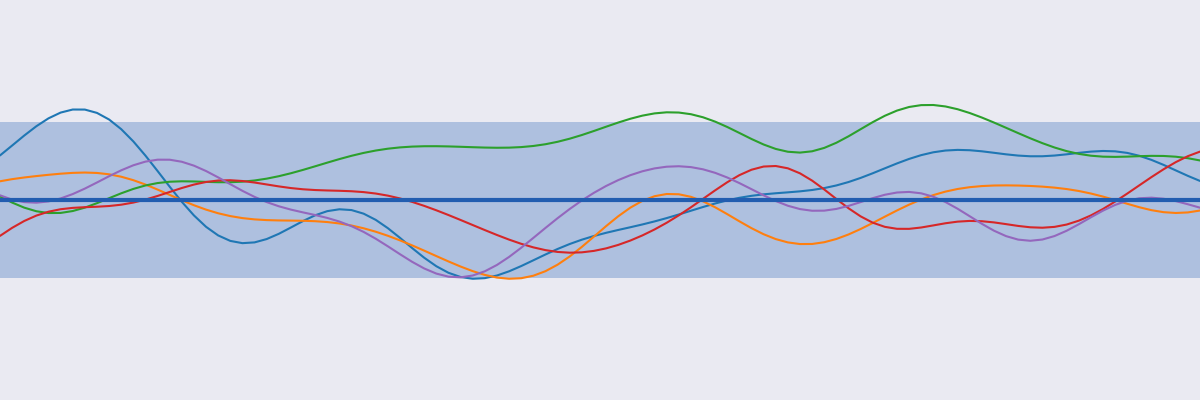
\includegraphics[width=\linewidth]{img_hyperopt/gp_prior.png}
	\caption[Gaussian process prior using a squared exponential kernel]{Gaussian process prior using a squared exponential kernel. The thin colored lines are samples drawn from the Gaussian process. The thick blue line represents the mean of the distribution and the blue area around this line is the $95 \%$ prediction interval, i.e. all drawn samples will be in this interval with a probability of $95 \%$ (for a Normal distribution this is equal to $1.96 \sigma$)}
	\label{fig:gp_prior}
\end{figure}

In probabilistic terms, the unfitted Gaussian process corresponds to the \textit{prior} probability $p \left( \mathrm{y} \right)$. Given a set of observed points $(\mathrm{X}, \mathrm{y})$ and a set of points we want to predict $(\mathrm{X_*}, \mathrm{y_*})$, the prior corresponds to $p\left( \mathrm{y_*} | \mathrm{X_*}, \theta \right)$, where $\theta$ denote the set of hyper-parameters of the covariance function. We are interested in the \textit{posterior} probability $p\left( \mathrm{y_*} | \mathrm{X_*}, \mathrm{X}, \mathrm{y}, \theta \right)$ i.e. the distribution of the new points conditioned on the points we have already observed. From probability theory we know that the posterior is:
\begin{equation}
    p\left( \mathrm{y_*} | \mathrm{X_*}, \mathrm{X}, \mathrm{y}, \theta \right)
    =
    \frac{p\left( \mathrm{y}, \mathrm{y_*} | \mathrm{X}, \mathrm{X_*}, \theta \right)}{p\left( \mathrm{y} | \mathrm{X}, \theta \right)}
    \label{eq:posterior}
\end{equation}
The numerator is called the \textit{joint distribution} and the denominator is the \textit{marginal likelihood}. 

\subsubsection{Inference}

Training a Gaussian process simply means pre-computing $K(\mathrm{X}, \mathrm{X})$, i.e. the covariance between the data points. At inference, we compute the covariance $K(\mathrm{X_*}, \mathrm{X_*})$ between the points we want to predict, and the covariance between the data points and the points we want to predict $K(\mathrm{X}, \mathrm{X_*})$. Since the covariance matrix is by definition symmetrical, $K(\mathrm{X_*}, \mathrm{X}) = K(\mathrm{X}, \mathrm{X_*})^T$. For notational simplicity we denote them $K$, $K_*$ or $K_*^T$ and $K_{**}$.

This results in the joint distribution of Equation~\ref{eq:posterior}:
\begin{equation}
    \begin{bmatrix}
    \mathrm{y} \\
    \mathrm{y_*}
    \end{bmatrix}
    \sim
    \mathcal{N} \left( 0, 
    \begin{bmatrix}
    K(\mathrm{X}, \mathrm{X}) & K(\mathrm{X}, \mathrm{X_*}) \\
    K(\mathrm{X_*}, \mathrm{X}) & K(\mathrm{X_*}, \mathrm{X_*})
    \end{bmatrix}
    \right)
    =
    \mathcal{N} \left( 0, 
    \begin{bmatrix}
    K & K_*^T \\
    K_* & K_{**}
    \end{bmatrix}
    \right)
\end{equation}
However the joint distribution generate functions that do not match the observed data. The posterior is obtained by conditioning the joint distribution to the observations, which are expressed by the marginal likelihood. Because every term involved is a Gaussian distribution, the posterior can be derived as follows:
\begin{equation}
    p\left( \mathrm{y_*} | \mathrm{X_*}, \mathrm{X}, \mathrm{y}, \theta \right)
    =
    \mathcal{N} \left( K_* K^{-1} y, 
    K_{**} - K_* K^{-1} K_*^T \right)
\end{equation}
This is the equation to compute when predicting new points. 

\begin{figure}[htb]
    \centering
    \begin{subfigure}[b]{\textwidth}
        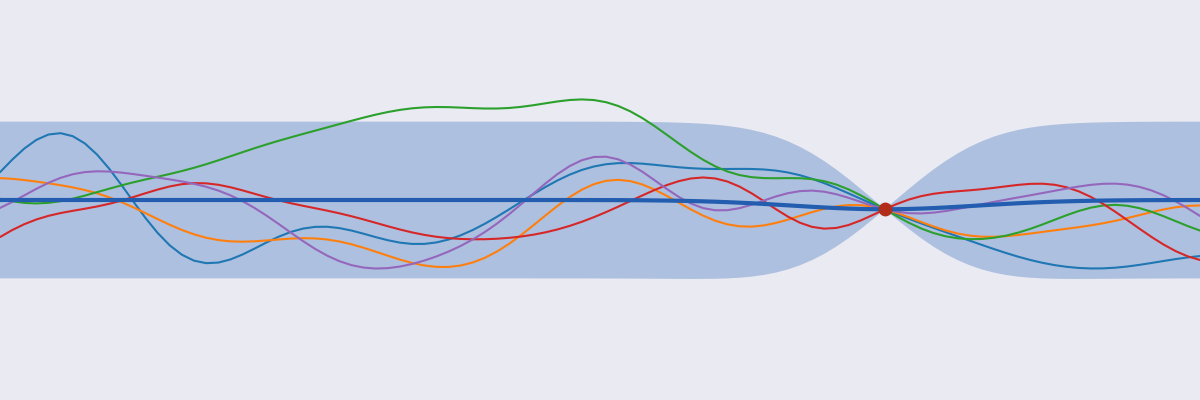
\includegraphics[width=\textwidth]{img_hyperopt/gp_posterior_1_point}
    \end{subfigure}

    \begin{subfigure}[b]{\textwidth}
        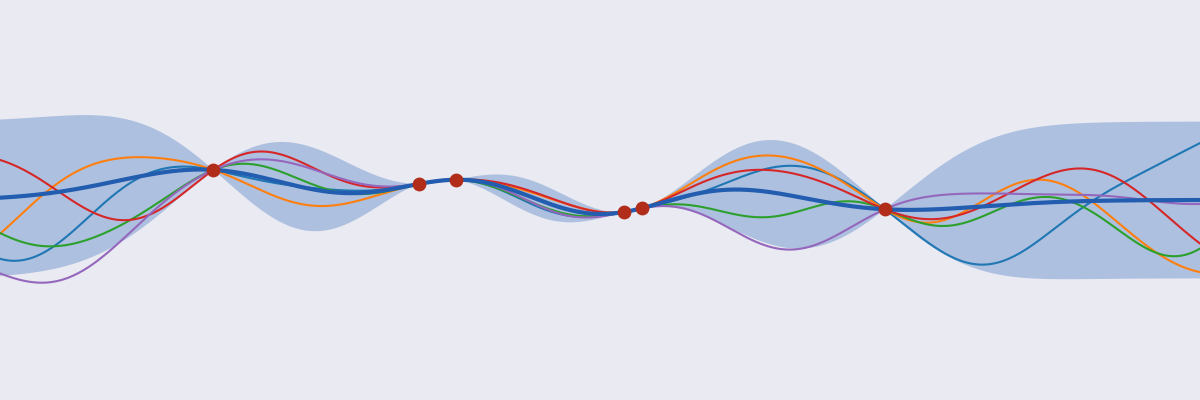
\includegraphics[width=\textwidth]{img_hyperopt/gp_posterior_6_point}
    \end{subfigure}
    \caption[Gaussian process posterior]{Gaussian process posterior after fitting one point on top, six on the bottom. All the samples pass through those points and the variance is lower close to them.}
    \label{fig:gp_posterior}
\end{figure}

Figure~\ref{fig:gp_posterior} shows how samples from this distribution look like on a one dimensional problem. Each sample must go through every observed point, and the closer the points are, the less freedom the samples have to change. Outside of the range of observed points, the distribution quickly reverts to its prior. 

%So far we have assumed for simplification that the data is noise-free, however it is important to note that Gaussian processes are particularly well-adapted for dealing with noisy data. See~\textcite{rasmussen2005} for the changes to the equations.

\subsubsection{Kernels}

The most common kernel is the squared exponential kernel:
\begin{equation}
	k(\mathrm{x}, \mathrm{x'}) = \sigma^2 \exp\left( -\frac{||\mathrm{x} - \mathrm{x'}||_2^2}{2l^2}\right)
	\label{eq:sqexp}
\end{equation}
With this kernel, the influence of a point on the value of another point decays exponentially with their relative distance. This implies that the Gaussian process quickly reverts to its prior in areas without observed points.

This kernel has two hyper-parameters $\theta = \{ \sigma^2 , l \}$. $\sigma^2$ controls the scale of the predicted output and $l$ is a vector of same dimensionality as $\mathrm{x}$ called the characteristic length-scale which measures how much a change along each dimension affects the output. A low value means that a small change in the input results in a big change in the output, as shown in Figure~\ref{fig:gp_lengthscale}. 

\begin{figure}[htb]
    \centering
    \begin{subfigure}[b]{\textwidth}
        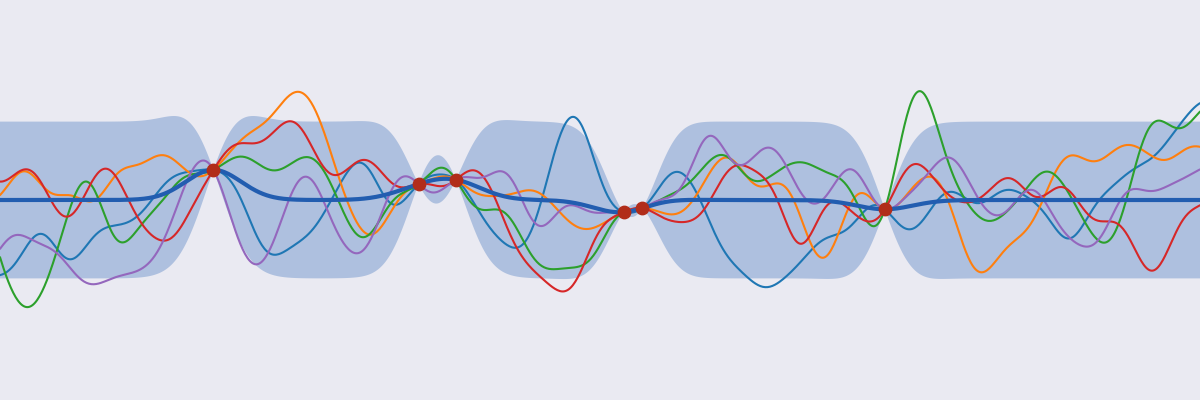
\includegraphics[width=\textwidth]{img_hyperopt/gp_lengthscale_small}
        \caption{$l = 0.3$}
    \end{subfigure}

    \begin{subfigure}[b]{\textwidth}
        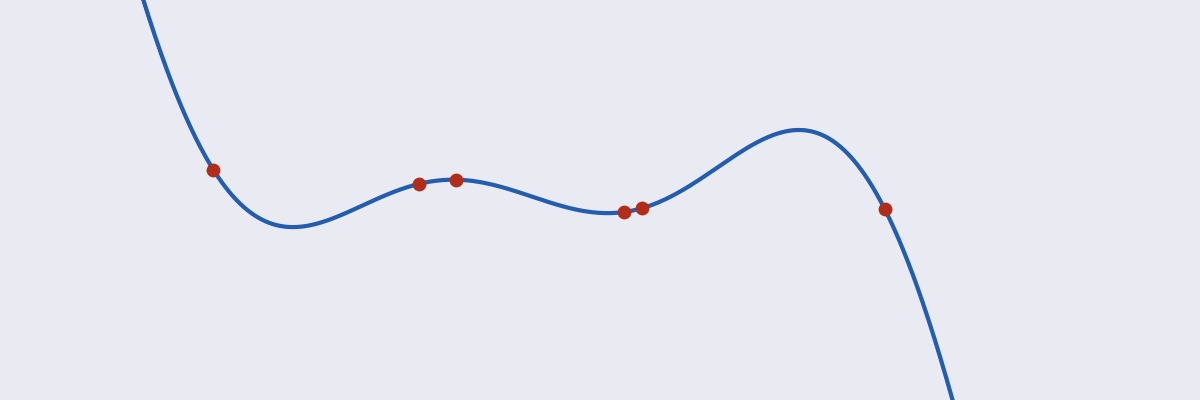
\includegraphics[width=\textwidth]{img_hyperopt/gp_lengthscale_big}
        \caption{$l = 3$}
    \end{subfigure}
    \caption[Gaussian process posterior with different length-scale]{Gaussian process posterior after six points with different length-scale. On the top with a low length-scale, data points are almost irrelevant, the Gaussian process returns to its prior almost immediately. On the bottom, the GP has a very high confidence in its prediction.}
    \label{fig:gp_lengthscale}
\end{figure}

The squared exponential kernel is a special case of the Matérn family of covariance functions which are, noting $r = || \mathrm{x} - \mathrm{x'} ||_2$ defined as follows:
\begin{equation}
    k_{\nu}(r) = \sigma^2 \frac{2^{1-\nu}}{\Gamma(\nu)} \left( \sqrt{2\nu} \frac{r}{l}\right)^{\nu} B_{\nu} \left( \sqrt{2\nu} \frac{r}{l}\right)
\end{equation}
$\Gamma$ is the gamma function and $B_{\nu}$ is the modified Bessel function of the second kind. The hyper-parameters $\sigma^2$ and $l$ are the same as for the squared exponential kernel and $\nu$ is a measure of how smooth the function is. $\nu = 1/2$ results in a very rough function while $\nu \to \infty$ is the squared exponential kernel.

The samples from the squared exponential kernel are very smooth, and are in fact infinitely differentiable. This is usually too unrealistic for the process we are modelling. In the context of Bayesian optimization, a more realistic alternative is the Matérn $5/2$ kernel:
\begin{equation}
    k(r) = \sigma^2 \left( 1 + \frac{\sqrt{5}r}{l} + \frac{5r^2}{3l^2} \right) \exp \left( - \frac{\sqrt{5}r}{l}\right)
\end{equation}
The chosen value of $\nu = 5/2$ means that the samples will be twice differentiable, which is a good compromise between too smooth and too difficult to optimize $\theta$, as many point estimate methods require twice differentiability (\textcite{snoek2012NIPS}). Figure~\ref{fig:gp_matern} shows what samples from these kernels look like.

\begin{figure}[htb]
    \centering
    \begin{subfigure}[b]{\textwidth}
        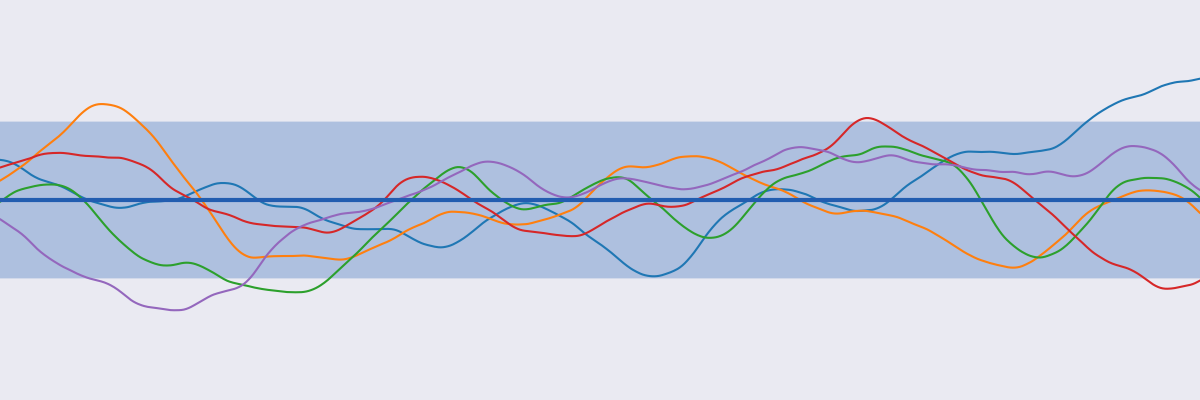
\includegraphics[width=\textwidth]{img_hyperopt/gp_matern_prior}
    \end{subfigure}

    \begin{subfigure}[b]{\textwidth}
        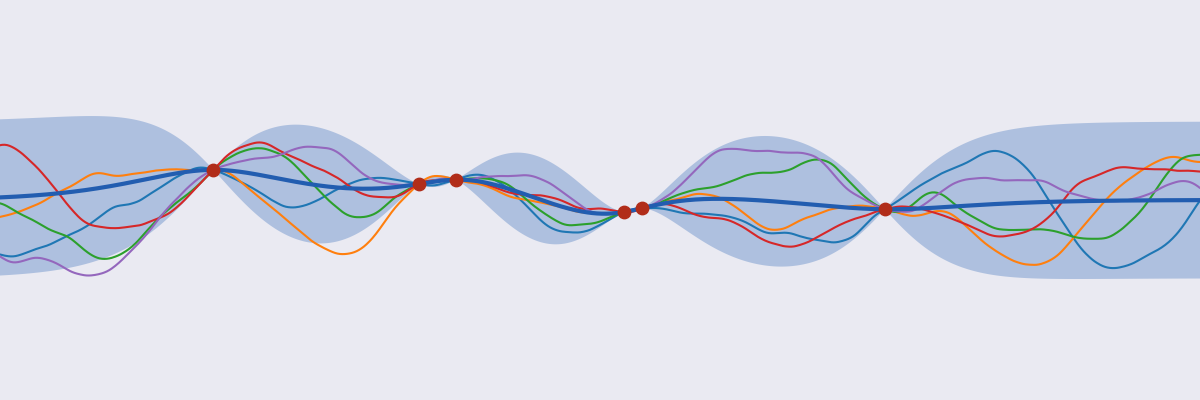
\includegraphics[width=\textwidth]{img_hyperopt/gp_matern_posterior}
    \end{subfigure}
    \caption[Gaussian process using a Matérn $5/2$ kernel]{Gaussian process using a Matérn $5/2$ kernel. On the top, the prior. On the bottom, the posterior after fitting six points.}
    \label{fig:gp_matern}
\end{figure}

The presented kernels have the common property of being stationary, i.e they depend only of $\mathrm{x} - \mathrm{x'}$. They are invariant to translation. It is particularly relevant in the context of hyper-parameter optimization as the kernels make no difference between values of 3 and 2 or 1000 and 999. For hyper-parameters where such a difference matters should use a non-stationary kernel instead of the ones presented above (see~\textcite{paciorek2003NIPS}).

\subsubsection{Learning the kernel hyper-parameters}

Kernels have themselves hyper-parameters $\theta$ which need to be chosen. For example, the squared exponential kernel has $l$, the characteristic length-scale. As shown by~\textcite{neal1996phd}, the inverse of the length-scale determines how relevant an input is. In the context of hyper-parameter optimization, it can help to choose which hyper-parameters to tune carefully. It is therefore very important to select a good value for $l$. 

There are two ways to learn $\theta$. The first way is to maximize the marginal likelihood, which can be derived as:  
\begin{equation}
	\log p\left(\mathrm{y} | \mathrm{X}, \theta \right) = - \frac{1}{2} \mathrm{y}^T K^{-1} \mathrm{y} - \frac{1}{2} \log |K| - \frac{n}{2} \log 2 \pi
\end{equation}
The optimization can be done with any off-the-shelf method, eventually with multiple restarts as there are no guarantee of a unique optimum. 
%For example, the scikit-learn (\textcite{pedregosa2011sklearn}) implementation uses BFGS with 10 restarts by default.

The other solution is to not learn $\theta$ at all and instead marginalize the hyper-parameters, i.e. at the inference step compute:
\begin{equation}
    p\left( \mathrm{y_*} | \mathrm{X_*}, \mathrm{X}, \mathrm{y} \right)
    = \int p\left( \mathrm{y_*} | \mathrm{X_*}, \mathrm{X}, \mathrm{y}, \theta \right) p \left( \theta | \mathrm{X}, \mathrm{y} \right) d\theta
\end{equation}
This integral is usually intractable but can be approximated by sampling methods. \textcite{murray2010NIPS} use slice sampling, \textcite{garbuno2016CSDA} use asymptotically independent Markov sampling and \textcite{titsias2011} review different Monte Carlo methods used for this problem.

%%%%%%%%%%%%%%%%%%%%%%%%%%%%%%%%%%
\subsection{Acquisition functions}
\label{ssec:acqfunc}

In the context of Bayesian optimization, the Gaussian process gives for each set of hyper-parameters an estimation of the performance of the corresponding model and the uncertainty of the Gaussian process in its estimation. But we do not have a way to decide which model is the most interesting to train. Do we pick a model that will be slightly better than our best current model, i.e. where the Gaussian process gives low uncertainty, or do we pick a model with high uncertainty but which could have low performance? There is an exploration/exploitation trade-off to be found. It is the role of the acquisition function to determine which model to train.

The oldest acquisition function is the Probability of Improvement (\textcite{kushner1964}). It chooses the model which has the highest probability of having better results than a target, which is usually picked to be the loss of the current best model. The \textit{PI} is defined as below, where $\Phi$ is the Normal cumulative distribution function, $\mathrm{x}$ represents a given set of hyper-parameters, $y_*$ is the minimum loss found so far, $\mu$ is the mean returned by the Gaussian process and $\sigma$ the variance:
\begin{equation}
    PI(\mathrm{x}) = \Phi \left( \frac{y_* - \mu(\mathrm{x})}{\sigma(\mathrm{x})}\right)
\end{equation}
The problem with this function is that it is highly sensitive to the choice of target. The simplest choice is the minimum loss found so far, but the \textit{PI} will then sample models very close to the corresponding model completely ignoring exploration. A better target is how much to improve the minimum loss. But this choice is very inconvenient because we usually have no idea of how much better the performance can get. Should we try to find a model $1 \%$ better? $5 \%$? $25 \%$? If we pick too big an improvement, the function will simply select the models with the highest uncertainty.

Instead, we can use the Expected Improvement function (\textcite{schonlau1998},~\textcite{jones2001}) which builds on the Probability of Improvement as below where $\phi$ is the normal density function:
\begin{equation}
	EI(\mathrm{x})  = \sigma (\mathrm{x}) [u\Phi(u)+\phi(u)]
\end{equation}
with
\begin{equation}
	u = \frac{y_* - \mu(\mathrm{x})}{\sigma(\mathrm{x})}
\end{equation}
The Expected Improvement \textit{EI} is obtained by taking the expectation of the improvement function (\textcite{shahriari2016IEEE}), defined as:
\begin{equation}
	I(\mathrm{x}) = \left(y_* - \mu(\mathrm{x}) \right) \mathds{1} \left(y_* > \mu(\mathrm{x}) \right)
\end{equation}
This function is equal to $0$ if the predicted mean is less than the best loss found so far (which means that there is no improvement), otherwise it is proportional to the gap between the predicted mean and best loss. 

The Expected Improvement has a major advantage over the Probability of Improvement. The target is always the minimum loss found so far, meaning that there is no need to guess a threshold of improvement. 

%%%%%%%%%%%%%%%%%%%%%%%%%%%%%%%%%%
\subsection{Bayesian optimization algorithm}

In summary, Bayesian Optimization works as follows. Given a set of explored combinations and their associated models performance, a Gaussian process fitted on that set is used to predict the performance of untested combinations. Then, an acquisition function takes those predictions and decides which combination should be tested next. This combination is tested, added to the set of explored combinations, and the process is repeated as long as resources are available. This process can be seen in Figure~\ref{fig:bo} on a one-dimensional problem. 

\begin{figure}[htb]
	\centering
	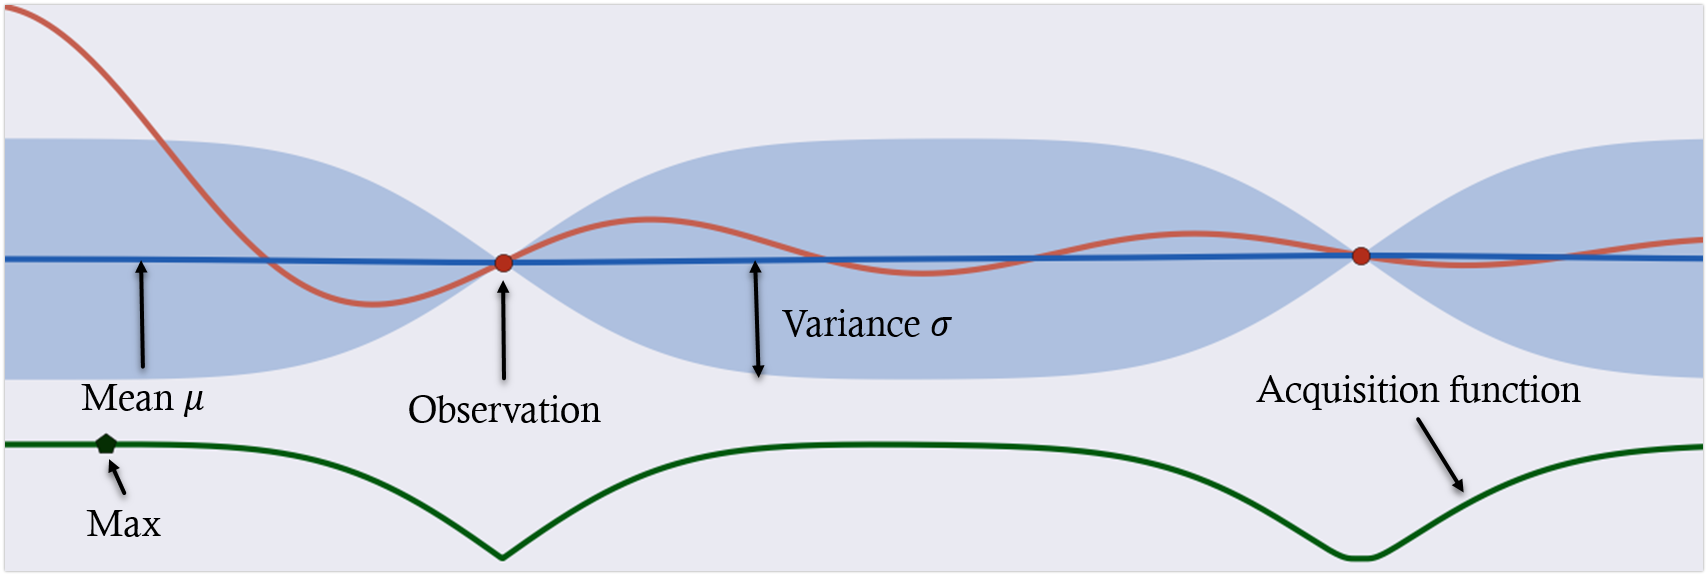
\includegraphics[width=\linewidth]{img_hyperopt/bo.png}
	\caption[Bayesian Optimization on a one dimensional function]{Bayesian Optimization on a one dimensional function. The orange curve is the true loss function, the blue one is the prediction of the Gaussian process. The green curve is the acquisition function. The next evaluation will be at the maximum of the green curve.}
	\label{fig:bo}
\end{figure}

%The process can be initiated by choosing the first model randomly or from a hand-crafted baseline when available.

%Some questions remain. How to pick the first model ? Select a random configuration of hyper-parameters from the hyper-parameter space. Should the Gaussian process predict the loss on the training set or on the validation set ? The loss on the validation set is to be preferred. How to sample configurations ? Uniformly from the hyper-parameter space. How many configurations should be sampled before selecting a model to train ? As many as reasonably possible. The step of selecting a model should be much faster than training it, and most of the cost of Bayesian optimization should be in the inversion of the Gram matrix (see Section~\ref{ssec:practical} for details).

%Hyperopt~\textcite{bergstra2013ICML}

%Practical~\textcite{snoek2012NIPS}

%%%%%%%%%%%%%%%%%%%%%%%%%%%%%%%%%%
% \subsection{Practical Challenges}
% \label{ssec:practical}

% %==One important aspect of this method is that the training time of the model is a dimension of the hyper-parameter space. This means that the method is free to choose how long to train each model. In practice we found that it prefers longer training time, even though it looks like a lower training time is enough to get a good estimate of the worth of the model and would allow the evaluation of more models. This is a flaw of the method, which lacks an explicit notion of budget and a way to best exploit it.

% \subsubsection{Conditional spaces}

% TODO
% \begin{itemize}
%     \item Describe cylindrical embeddings
%     \item Describe tree of Parzen estimator
% \end{itemize}

% The version of Bayesian optimization we presented deals efficiently with both discrete and continuous hyper-parameters. But what about conditional hyper-parameters ? For example, some hyper-parameters could be specific to a particular layer and one hyper-parameter could control the number of layers. But then, what happens to the hyper-parameters of a non-existent layer ? With a Gaussian process, we need to give them a value and it means there will be many configurations that corresponds to the same model. In practice, we can ignore those cases, and the Gaussian process will eventually give a low uncertainty in those regions and pick models elsewhere. But this is extremely wasteful as we will retrain the same model many times before this happens ! 

% One solution is to use a specialized kernel called a cylindrical kernel (\textcite{swersky2013},~\textcite{oh2018}).

% Another solution is to not use a Gaussian process at all. It has been our model of choice so far but other alternatives exist. One such alternative is tree-structured Parzen estimator (\textcite{bergstra2011NIPS}).

% \subsubsection{Parallelization}

% Open problem using GP

% See combination with Hyperband for a potential solution

% \subsubsection{Non-stationarity}
% \label{ssec:nosta}

% Input Warping~\textcite{snoek2014ICML}

% \subsubsection{Scaling}

% Doesn't work well in high-dimension or with thousands of data points

% Conditional neural processes ?

%%%%%%%%%%%%%%%%%%%%%%%%%%%%%%%%%%
\section{Incremental Cholesky decomposition}
\label{sec:cholesky}

\subsection{Motivation}
\label{ssec:motivation}

The costliest part of Bayesian optimization is the construction of the Gram matrix $K$ and the computation of its invert $K^{-1}$. To reduce that cost, the standard solution is to compute the Cholesky decomposition $L$ of the Gram matrix and invert the decomposition. Every time the Gram matrix is modified, the Cholesky decomposition and its inverse are fully recomputed.

However, Bayesian optimization alters the Gram matrix only by adding new rows and columns corresponding to the covariance between the $n$ older combinations and the $k$ new combinations. The Gram matrix can therefore be decomposed in blocks where one of them is the previous Gram matrix. By calling $K_{(n,n)}$ the previous matrix and $K_{(n+k,n+k)}$ the new one with the added points, the decomposition is:
\begin{equation}
	K_{(n+k,n+k)} = 
	\begin{pmatrix}
    K_{(n,n)} & K_{(k,n)}^T \\
    K_{(k,n)} & K_{(k,k)}
  \end{pmatrix}
\end{equation}
Likewise, the Cholesky decomposition and its inverse can also be decomposed into blocks where one is the previous Cholesky decomposition as we show in Section~\ref{ssec:formulas}. We then argue in Section~\ref{ssec:complexity} that this can be used to make Bayesian optimization faster by updating incrementally the Cholesky decomposition instead of fully recomputing it each time.

\subsection{The incremental formulas}
\label{ssec:formulas}

The derivation of both formulas can be found in Appendix~\ref{app:cholesky}. We present here only the final results. The formula of the incremental Cholesky decomposition is:
\begin{equation}
  L_{(n+k)} = 
  \begin{pmatrix}
    L_{(n)} & 0 \\
    K_{(k,n)} (L_{(n)}^T)^{-1} & L_{(k)}
  \end{pmatrix}
\end{equation}
Since this formula requires the costly computation of $L_{(n)}^{-1}$, we are also interested in an incremental formula for it, which is:
\begin{equation}
  L_{(n+k)}^{-1} =
  \begin{pmatrix}
    L_{(n)} & 0 \\
    K_{(k,n)} (L_{(n)}^T)^{-1} & L_{(k)}
  \end{pmatrix}^{-1} = 
  \begin{pmatrix}
    L_{(n)}^{-1} & 0 \\
    - L_{(k)}^{-1} K_{(k,n)} (L_{(n)}^T)^{-1} L_{(n)}^{-1} & L_{(k)}^{-1}
  \end{pmatrix}
\end{equation}

\subsection{Complexity improvement}
\label{ssec:complexity}

A standard Cholesky decomposition has a complexity of $O \left( (n + k)^3 \right)$ with $n + k$ the number of observed combinations. With our formulas, since we already have $L_{(n)}$, all that is left is to compute $L_{(k)}$, which has a cost of $O \left( k^3 \right)$. Since Bayesian optimization is called after every tested combination, $k = 1$, the Gram matrix just has one new row and one new column. $L_{(k)}$ and its inverse are trivial to compute.

There is however an increased cost in memory, as $L_{(n)}$ and $L_{(n)}^{-1}$ must be stored between calls of Bayesian optimization. They are two $n \times n$ triangular matrices, storing them cost $O \left( n^2 \right)$, which seems a reasonable price to pay for the performance improvement.

%%%%%%%%%%%%%%%%%%%%%%%%%%%%%%%%%%%%%%%%%%%%%%%%%%%%%%%%%%%%%%%%%%%%%%%%%%%%%%%%%%%%%%%%%%%%%%%
\section{Comparing Random Search and Bayesian Optimization}
\label{sec:compare}

In this section we study the theoretical performance of random search, before devising an experiment that compares the performance of random search and Bayesian optimization in a practical setting.

%%%%%%%%%%%%%%%%%%%%%%%%%%%%%%%%%%
\subsection{Random search efficiency}
\label{ssec:random}

How many models of a hyper-parameters space should be trained in order to be reasonably certain to have trained one of the best models? If we knew the loss $l_{min}$ of the best model, how long would it take to find a model with a loss such that $l \leq (1 + \alpha) l_{min}$? Due to the relative simplicity of random search, we can derive theoretical bounds to answer these questions.

Let $N$ be the total number of models in the hyper-parameters space, $M$ the number of models satisfying our performance criteria (alternatively, the $M$ best models of the space) and $n$ the number of models to train.

Considering that random search chooses models uniformly, the probability of drawing one of the best models the first time is simply $\frac{M}{N}$. The second time, it is $\frac{M}{N - 1}$ since we do not allow redrawing a model. We can therefore define the probability of not drawing any satisfying models after $n$ draws as the following equation, where $Y$ is the random variable of failing to draw an acceptable models among $n$ draws in a row.
\begin{equation}
    P \left( Y = n \right) = \prod_{k = 0}^{n} \left( 1 -  \frac{M}{N - k} \right)
\end{equation}
This is a particular case of the hypergeometric distribution. From there, the probability of drawing an acceptable model at the $n$-th draw is:
\begin{equation}
    P\left(X = n \right) = \frac{M}{N - n} \prod_{k = 0}^{n - 1} \left( 1 -  \frac{M}{N - k} \right)
\end{equation}
$X$ is the random variable of drawing an acceptable model after $n - 1$ bad draws. The probability of drawing an acceptable model in the first $n$ draws is:
\begin{equation}
    P\left(X \leq n \right) = \sum_{k = 0}^{n} P\left(X = k \right)
\end{equation}
From this equation we can compute the number of draws required to have drawn a model in the top $\alpha \%$, by setting $M$ as a fraction of $N$. Moreover since the equation depends only of the ratio $\frac{M}{N - k}$, the effect of $k$ becomes negligible as $N$ grows bigger and the equation converges.

\begin{table}[htb]
	\centering
	\begin{tabular}{ | l | c | c | c | }
		\hline
		 & $p > 0.5$ & $p > 0.95$ & $p > 0.99$ \\ 
		\hline
		Top $1 \%$ & 69 & 298 & 458 \\
		Top $5 \%$ & 14 & 59 & 90 \\
		Top $10 \%$ & 7 & 29 & 44 \\
		\hline
	\end{tabular}
	\caption[Theoretical performance of random search]{Number of draws required to have drawn a model in the top $\alpha \%$ with probability $p$ in a space of 100 000 combinations.}
	\label{table:random_search_bounds}
\end{table}

In Table~\ref{table:random_search_bounds}, we present some of those results, which allow us to draw the following strong conclusion. For any hyper-parameter space, random search will draw a model in the top $5 \%$ of models in 90 draws with a probability of $99 \%$. Less than a hundred draws is sufficient to draw one of the best models of any hyper-parameter space. It is a surprisingly low number given the simplicity of the method.

However that is only one of the questions we asked. Ranking the models by their performance does not guarantee that a model in the top $\alpha \%$ is within $\alpha \%$ of the performance of the best model (i.e. whose performance verifies $l \leq (1 + \alpha) l_{min}$), unless model performance happens to be uniformly distributed. Since we have no idea of how model performance is distributed, we cannot go further in our theoretical analysis. In Section~\ref{ssec:cifar_analysis}, we return to this question by studying empirically the distribution of model performance.

%%%%%%%%%%%%%%%%%%%%%%%%%%%%%%%%%%
\subsection{Bayesian optimization efficiency}

While we were not able to obtain similar results for Bayesian optimization as we did for random search, we expose some of the difficulties in doing so.

First any analysis depends of the exact setup of Bayesian optimization. A change of kernel or acquisition function changes the results. But the main problem is that, because the process learns the structure of the hyper-parameter space, any analysis would need to work in a particular space.

None of those difficulties prevent us from measuring the empirical performance of Bayesian optimization, as we show in the next section.

%%%%%%%%%%%%%%%%%%%%%%%%%%%%%%%%%%
\subsection{Experiments on CIFAR-10}
\label{ssec:cifar_analysis}

\subsubsection{Setup}

In order to compare the performance of the different hyper-parameter optimization methods, we devised a hyper-parameter space containing 600 models and trained them all on the CIFAR-10 dataset (\textcite{krizhevsky2009}).

The dataset is composed of 60 000 images equally divided in 10 classes. The images are 32x32 RGB images. The training set contains 50 000 images, the test set 10 000.

Since the goal of the experiment is not to beat the state-of-the-art on the dataset, the selected hyper-parameter space and the resulting models are small and simple. Each model is trained for a total of 10 minutes on a NVIDIA TITAN X card. 

We then compare in which order the different methods selected the models. The methods are evaluated on the time needed to select the best model, as well as the time needed to select a model in the top $\alpha \%$.
%but also on the average performance of the selected models, i.e. if we rank the models by their performance, how close was each method from selecting the models in that order.

However one run is not enough to conclude that Bayesian optimization on average is more efficient than random search. Due to the huge computing cost, we cannot do hundreds of runs with different seeds and retrain each network every time. But if we do not retrain the network but change the seeds of the search policy, we can simulate hundreds of runs at a low cost. 

There are a total of $600!$ way to explore this space, but because we do not retrain the models, all the randomness in Bayesian optimization is in the choice of the first model\footnote{This is true for our specific approach. Incorporating Gaussian noise in the observations ($\hat{y} = y + \mathcal{N} \left( \mu, \sigma)\right)$) for example would make our analysis incorrect.}, leaving us with only 600 possible paths through this space. We computed them all, then randomly selected 600 ordering for random search.

\subsubsection{Models distribution}

\begin{figure}[htb]
	\centering
	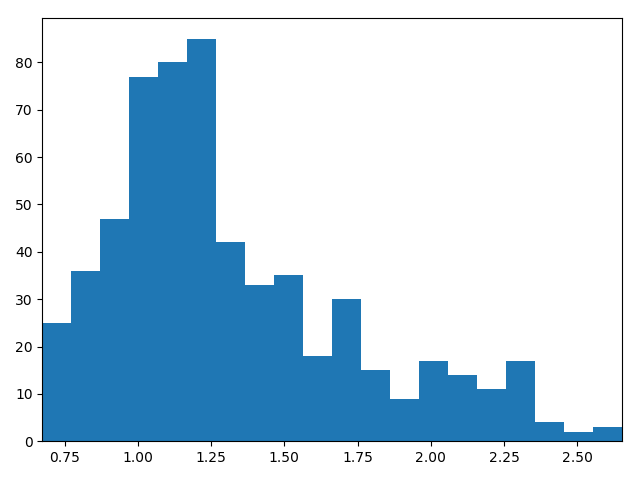
\includegraphics[width=0.7\linewidth]{img_hyperopt/cifar_hist.png}
	\caption{Distribution of the models performance.}
	\label{fig:cifar_hist}
\end{figure}

Before comparing the search methods, we look at the distribution of models performance in Figure~\ref{fig:cifar_hist}. A few models are really good, most are average and then there is a long trail of progressively worse models. It looks like a skew normal distribution. 

We cannot extrapolate that every hyper-parameter space will have a distribution like this, but we assume for now that this is the case for hyper-parameter spaces designed in practice.

Since the distribution is not uniform, there is a difference between models in the top $5 \%$ of models and models that have a performance within $5 \%$ of the performance of the best model. In this case, there are 30 models in the top $5 \%$ of models (since there are 600 models), but only 6 are within $5 \%$ of the performance of the best model. In this case, the 30-th best model is within $18 \%$ of the best model.

This distinction is important because it changes our evaluation of the methods. We are not simply interested in the average time to find a model in the top $\alpha \%$ of models, but also in the average time to find a model within $\alpha \%$ of the best model.

\subsubsection{Results}

\begin{figure}[htbp]
	\begin{subfigure}[b]{\textwidth}
            \centering
            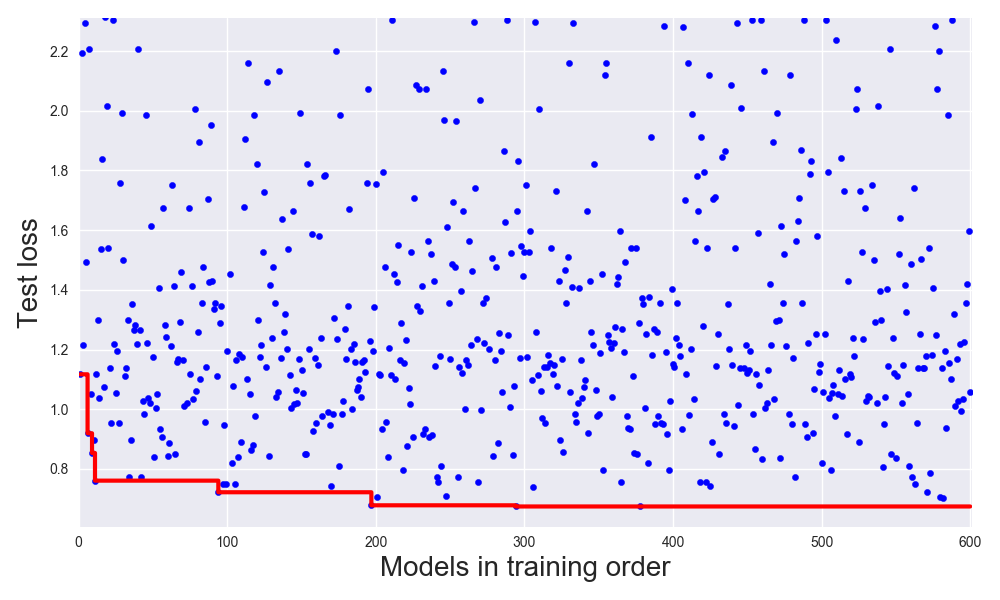
\includegraphics[width=\linewidth]{img_hyperopt/cifar_random}
    \end{subfigure}%
    
    \begin{subfigure}[b]{\textwidth}
            \centering
            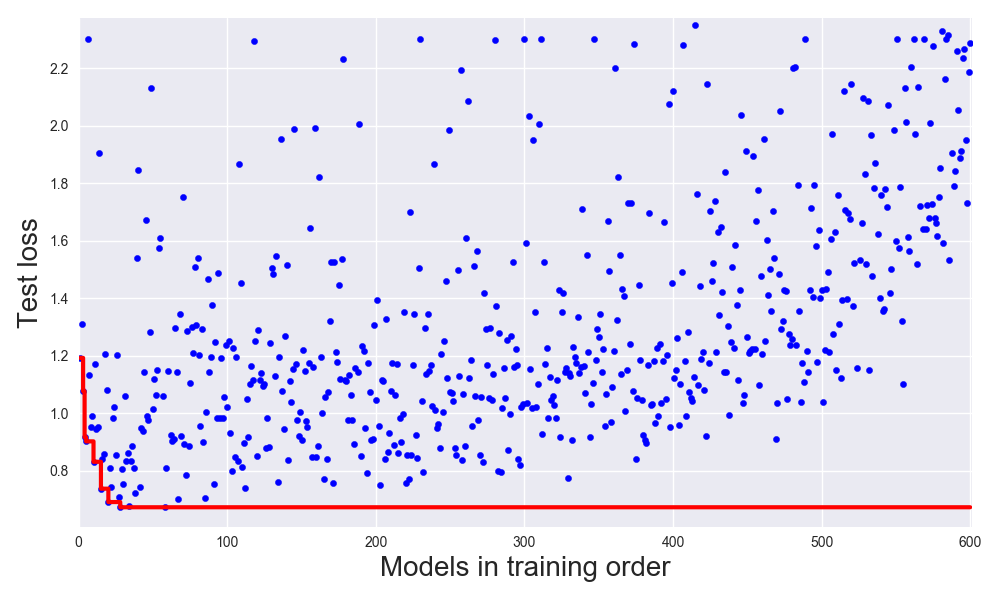
\includegraphics[width=\linewidth]{img_hyperopt/cifar_bo}
    \end{subfigure}%
    \caption[Comparing random search and Bayesian optimization]{Comparing the model order chosen by random search (top) vs Bayesian optimization (bottom).}
	\label{fig:cifar_loss}
\end{figure}

First, we look at the order in which models where selected during one run, shown in Figure~\ref{fig:cifar_loss}. The blue points represent the test loss of the models in the order the methods selected them, and the red line shows the minimum loss found at a given time. There is a clear trend present for Bayesian optimization where the combinations evaluated later have low performance, suggesting it did learn to predict correctly the performance of untested combination. In this run, it was also able to find the best model much earlier than random search. Random search behaves as expected and models performance is uniformly distributed.

\begin{table}[htb]
	\centering
	\begin{tabular}{ | l | c | c | c | c | }
		\hline
		 & \multicolumn{2}{|c|}{Random Search} & \multicolumn{2}{|c|}{Bayesian optimization} \\ 
		%\hline
		& Average & Worst & Average & Worst \\
		\hline
		Best model & $297 \pm 171$ & $599$ & $87 \pm 64$ & $249$ \\
		\hline
		Within $1 \%$ & $146 \pm 114$ & $554$ & $26 \pm 16$ & $120$ \\
		Within $5 \%$ & $87 \pm 75$ & $397$ & $17 \pm 11$ & $67$ \\
		Within $10 \%$ & $54 \pm 52$ & $296$ & $15 \pm 9$ & $44$ \\
		\hline
		Top $1 \%$ & $87 \pm 75$ & $397$ & $17 \pm 11$ & $67$ \\
		Top $5 \%$ & $18 \pm 17$ & $106$ & $10 \pm 8$ & $38$ \\
		Top $10 \%$ & $10 \pm 10$ & $62$ & $7 \pm 7$ & $36$ \\
		\hline
	\end{tabular}
	\caption[Average and worst number of draws taken by each method to reach different goals over 600 runs]{Average and worst number of draws taken by each method to reach different goals over 600 runs. Within $\alpha \%$ mean within $\alpha \%$ of the performance of the best model.}
	\label{table:search_average}
\end{table}

To confirm these trends, we look at the average number of draws taken by each method to reach different goals (Table~\ref{table:search_average}).

Random search needed on average 297 draws before finding the best model, which is within the expected range of the theoretical value of 300 draws. If we rank the model by their performance, random search needed an average of 18 draws to find a model in the top $5\%$ and 87 to find a model in the top $1\%$.

In comparison, Bayesian optimization did a lot better on every goal. On average it needed 87 draws to find the best model and only 17 to find a model in the top $1 \%$. In most cases the worst run of Bayesian optimization performed better than the average run of random search.

\begin{figure}[htb]
	\centering
	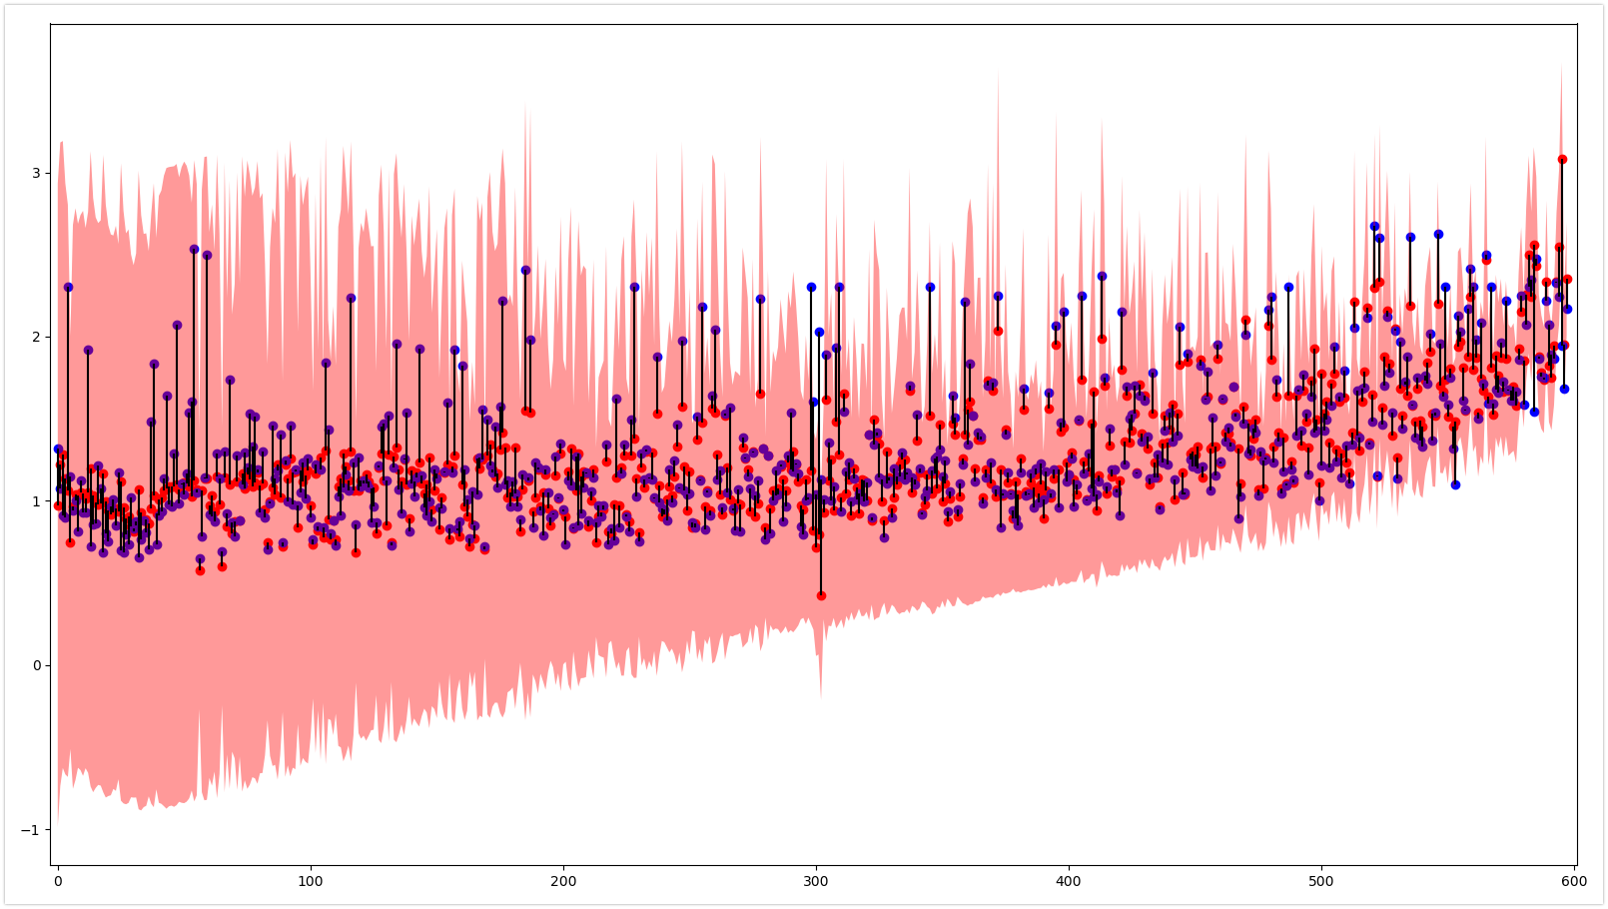
\includegraphics[width=\linewidth]{img_hyperopt/bo_error_time.png}
	\caption[Model performance predicted by the Gaussian process vs the true performance]{Model performance predicted by the Gaussian process in red vs the true performance in blue. The colored area is the $95 \%$ prediction interval.}
	\label{fig:bo_error_time}
\end{figure}

To confirm whether the Gaussian process is learning the structure of the hyper-parameter space, Figure~\ref{fig:bo_error_time} shows the predicted performance and the true performance, as well as the $95 \%$ prediction interval. As more models are used to refine the Gaussian process, the prediction interval shrinks, i.e. the Gaussian process becomes more confident in its prediction. Prediction for outliers, in this case models that do not learn, is highly inaccurate at the beginning and is still the main source of error at the end.

\subsection{Conclusion}

We designed an experiment to measure and compare the performance of random search and Bayesian optimization on a setting mimicking real life usage. Performance of random search matched closely theoretical results, showing the surprising efficiency of this method. Bayesian optimization outperformed random search on every metric, which justifies its much higher implementation cost.

Extending the hyper-parameter space would yield insights into how Bayesian optimization behaves in larger spaces. This framework of testing could be used to observe the behaviour of other methods such as Hyperband. We observed models performance to be normally distributed, but the scope is limited to one hyper-parameter space on one task. To the best of our knowledge there is no theory on how to build good hyper-parameter spaces and understanding the relation between models, tasks and model performance would be of practical use to the design of hyper-parameter optimization methods.

%%%%%%%%%%%%%%%%%%%%%%%%%%%%%%%%%%%%%%%%%%%%%%%%%%%%%%%%%%%%%%%%%%%%%%%%%%%%%%%%%%%%%%%%%%%%%%%
\section{Combining Bayesian Optimization and Hyperband}
\label{sec:cap}

This section describes and extends the work presented at CAp 2017 (\textcite{bertrand2017CAp}). We propose a new method of hyper-parameter optimization that combines Bayesian optimization and Hyperband.

%%%%%%%%%%%%%%%%%%%%%%%%%%%%%%%%%%
\subsection{Hyperband}
\label{ssec:hyperband}

A property of neural networks is that their training is usually iterative, usually some variant of gradient descent. A consequence is that it is possible to interrupt training at any time, evaluate the network, then resume training. This is the property Hyperband (\textcite{li2017ICLR}) takes advantage of.

The principle is simple: pick randomly a group of configurations from a uniform distribution, train the corresponding networks partially, evaluate them, resume training of the most performing ones, and continue on until a handful of them have been trained to completion. Then pick a new group and repeat the cycle until exhaustion of the available resources.

But a problem appears: at which point in the training can we start evaluating the models? Too soon and they will not have started to converge, making their evaluation meaningless, too late and we have wasted precious resources training under-performing models. Moreover, this minimum time before evaluation is hard to establish and changes from one task to the other. Some hyper-parameters (such as the learning rate) even influence the training speed! Hyperband's answer is to divide a cycle into brackets. Each bracket has the same quantity of resource at its disposal. The difference between brackets is the point at which they start evaluating the models. The first bracket will start evaluating and discarding models very early, allowing it to test a bigger number of configurations, while the last bracket will test only a small number of configurations but will train them until the maximum number of resources allowed per model.

The algorithm is controlled by two hyper-parameters: the maximal quantity of resources $R$ that can be allocated to a given model, and the proportion of configurations $\eta$ kept at each evaluation. $R$ is typically specified in number of epochs or in minutes. At each evaluation, $1 / \eta$ models are kept while the rest are discarded. 

%%%%%%%%%%%%%%%%%%%%%%%%%%%%%%%%%%
\subsection{Combining the methods}

Bayesian optimization and Hyperband being orthogonal approaches, it seems natural to combine them. Hyperband chooses the configurations to train uniformly and intervenes only during training. On the other side, Bayesian optimization picks configurations carefully by modelling the loss function, then let them train without interruption.

As a result, Hyperband does not improve the quality of its selection with time, while Bayesian optimization regularly loose time training bad models.

Combining the methods fixes these problems. Model selection is done by Bayesian optimization as described in Section~\ref{sec:bo}, then Hyperband train them as described in Section~\ref{ssec:hyperband}. Two changes are required for Bayesian optimization, as it needs some way to distinguish between fully-trained models and partially trained models. To do that, the training time becomes an hyper-parameter, making the performance of each model at every minute a distinct point. The performance prediction is then done at the training time corresponding to Hyperband's first evaluation, to have only one prediction per model.

The second change is to normalize the values returned by the acquisition function to make it a probability distribution, i.e. divide each value by the sum of all values, so that the sum of all normalized values is equal to one. In the standard usage of Bayesian optimization, the chosen model is the argmax of the acquisition function. Choosing the top $\alpha$ models yields models that are very close as the acquisition function is smooth and gives similar values for nearby combinations. This strategy removes the property of Hyperband to explore many regions of space at the same time. Normalizing the values and drawing from this distribution keeps this property, while making the selection smarter over time as it changes to reflect the knowledge acquired from the trained models.

The proposed algorithm is as follows: the first group of configurations is chosen randomly and evaluated according to Hyperband. All subsequent selections are done by training a Gaussian process with a squared-exponential kernel on all evaluated models. The expected improvement is then computed on all untested combinations and normalized to make a probability distribution from which the next group of models is sampled.

%%%%%%%%%%%%%%%%%%%%%%%%%%%%%%%%%%
\subsection{Experiments and results}

We compare the three methods presented above: Bayesian optimization, Hyperband, and Hyperband using Bayesian optimization. The algorithms were implemented in Python using scikit-learn (\textcite{pedregosa2011sklearn}) for the Gaussian processes and Keras (\textcite{chollet2015keras}) as the deep learning framework.

Comparison was done on the CIFAR-10 dataset (\textcite{krizhevsky2009}), which is a classification task on $32 \times 32$ images. The image set was split into $50\%$ for the training set used to train the neural networks, $30\%$ for the validation set used for the Bayesian model selection and the rest as test set used for the reported results below. 

Each method is allocated a total budget $B = 4000$ minutes meaning the sum of all the models training time must be equal to 4000 at the end of the process. The choice of having a budget in time means that models will not be trained in epochs as usual, but in minutes. This is a practical choice that allows estimating accurately the total time that the search takes, though it has the effect of favoring small networks. Indeed, two models trained an equal amount of time will not have seen an equal amount of data if one model is bigger and thus slower than the other. The choice to constrain in time instead of epoch means that the quantity of data seen by the models depends on the GPU. The training is done on two NVIDIA TITAN X.

\begin{table}[htbp]
	\centering
	\begin{tabular}{ | l | c | }
		\hline
		Hyper-parameter & Range of values \\ \hline
		Number of convolutional blocks & $\left[ 1; 5\right]$ \\
		Number of convolutional layers per block & $\left[ 1; 5\right]$ \\
		Number of filters per layer & $\left[ 2; 7\right]$ \\
		Filter size & $\left\{ 3; 5; 7; 9 \right\}$ \\
		Learning rate & $\left\{ 10^{-5}; 10^{-4}; 10^{-3}; 10^{-2} \right\}$ \\
		Batch size & $\left[ 2; 9\right]$ \\
		\hline
	\end{tabular}
	\caption{Hyper-parameter space explored by the three methods.}
	\label{table:hyperspace_combine}
\end{table}

The chosen architecture is a standard convolutional neural network with varying number of layers, number of filters and filter size per layer. Other hyper-parameters involved in the training method are: the learning rate, the batch size and the presence of data augmentation. In total there are 6 hyper-parameters to tune for a total of 19 200 possible configurations, displayed in Table~\ref{table:hyperspace_combine}.

For Hyperband, we chose $R = 27$, meaning 27 models are chosen at each iteration and are trained for a maximum of 27 minutes, and $\eta = 3$ which means that $1/3$ of the models are kept at each evaluation. In the case of Bayesian optimization, each model was trained $30$ minutes but they are chosen sequentially.

\begin{figure}[htb]
	\begin{minipage}[b]{.49\linewidth}
		\centering
		\centerline{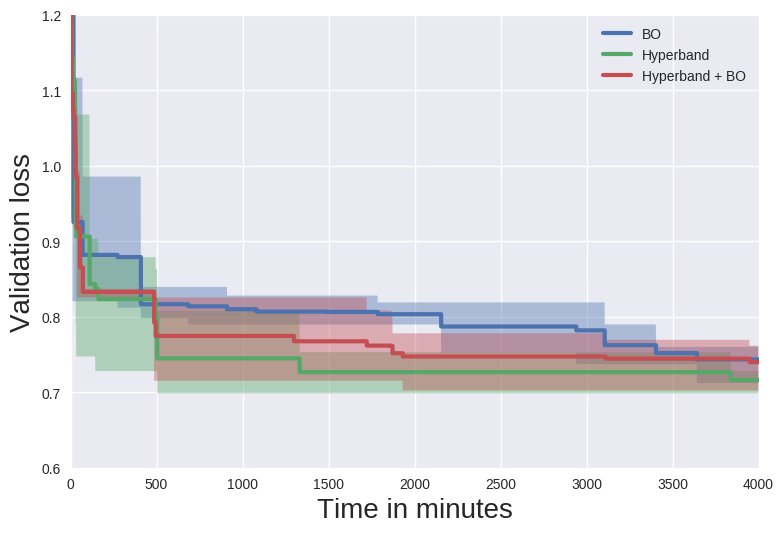
\includegraphics[width=7.2cm]{img_hyperopt/cifar_10_aggregate_best_val_loss_per_minute}}
	\end{minipage}
	\begin{minipage}[b]{.49\linewidth}
		\centering
		\centerline{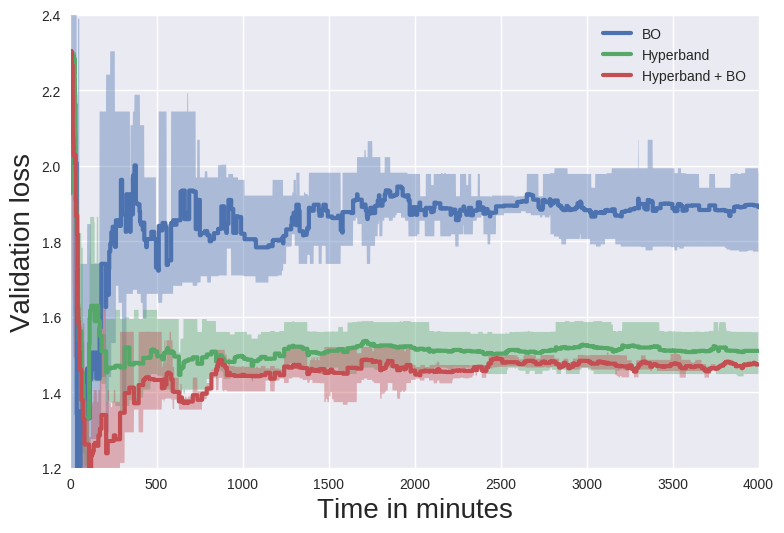
\includegraphics[width=7.2cm]{img_hyperopt/cifar_10_aggregate_median_val_loss_per_minute}}
	\end{minipage}
	\caption[Loss of the best model and running median of the loss as the methods progress]{(Left) Loss of the best model found at a given time by each method. (Right) Running median of the loss of all tested models for each method.}
	\label{fig:combining_loss}
\end{figure}

The evaluation measure that matters when comparing methods is the loss of the best model found at a given time, and is illustrated in Figure~\ref{fig:combining_loss} for the two individual methods and their combination (5 runs each). 
The running median suggest that Bayesian optimization (in blue) performs slightly worse than both other methods, and that Hyperband with Bayesian optimization (in red) finds a better model quicker than Hyperband (in green). However, due to the stochastic nature of the methods, many more runs would be needed to draw definite conclusions from this evaluation measure. 

It is more informative to look at the running median of the loss of all models trained at a given time, as it gives us an idea of the quality of the models tried as the methods progress. Ideally the running median should go down for Bayesian optimization and Hyperband as more models are tested and the methods either learn the shape of the space or stop training inefficient models. Bayesian optimization performs notably worse than the other two methods. Hyperband and Hyperband + BO have similar performance, though Hyperband + BO seems slightly better.

%%%%%%%%%%%%%%%%%%%%%%%%%%%%%%%%%%
\subsection{Discussion}

Due to the part of chance in all three methods, five runs are not enough to draw definite conclusions on their performance. Ideally hundreds of runs would have been needed, and the computational cost of this endeavor was the main reason we did not pursue further this problem. At 4000 minutes per method per seed, the above experiment already required around 42 days of GPU time without accounting for the overhead (loading the data, building the models, ...).

While the general idea of combining Hyperband and Bayesian optimization is valid, there are two problems with our specific approach. 

As mentioned previously, since Bayesian optimization is usually sequential, we normalized the results of the acquisition function to make it a probability distribution from which the models to train were sampled. However the resulting distribution was very close from a uniform distribution. This is because the expected improvement outputs values in a small range, i.e. the difference between the maximum and the minimum is at most a few orders of magnitude. When normalized, those extreme values would not be particularly likely, even with just a small hyper-parameters space of $19 200$ combinations. For example if the highest value is a hundred times the average value, after normalization, the corresponding model has only around $0.5\%$ chance of being sampled. This is why our version of Hyperband + BO performed barely better than Hyperband alone. 

One potential solution is to use the "liar" strategy. After choosing a model but before training it, it is added to the training set with a low performance and the acquisition function is re-computed. The "lie" of the low performance discourages the acquisition function from giving high values to the surrounding models, and the argmax will be a completely different model. Repeating this process allows drawing many models simultaneously. 

When drawing a large group of models at the same time as required by Hyperband, the cost of this process becomes important as the Gram matrix of the Gaussian process needs to be inverted many times. The incremental Cholesky decomposition presented in Section~\ref{sec:cholesky} could be used to make the process faster.

\begin{figure}[htbp]
	\centering
	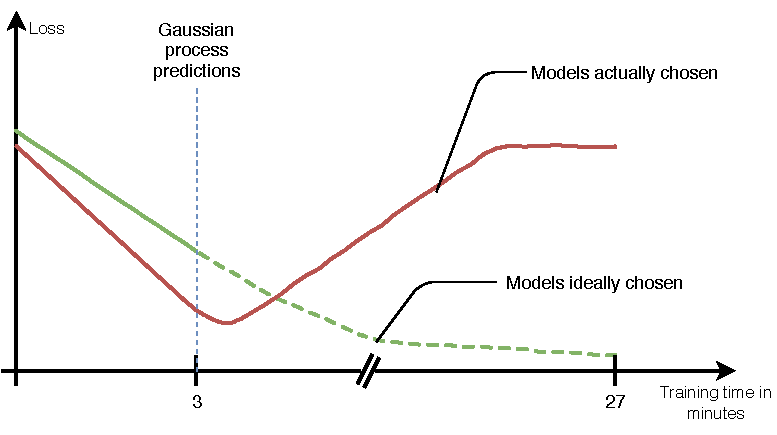
\includegraphics[width=\linewidth]{img_hyperopt/combine_overfit}
	\caption[Why predicting model performance at 3 minutes lead to overfitting]{The problem with predicting model performance at 3 minutes (dotted blue line). Models that trained faster (due to being smaller, red line) have better performance at 3 minutes than bigger models (green line), however they overfit shortly after while the bigger models end up with a better performance.}
	\label{fig:combine_overfit}
\end{figure}

Informal observations of the chosen models revealed a second problem. After a few iterations, many of the models chosen tended to have converged to their best performance by the time of Hyperband's first evaluation (after 3 minutes of training) and to start overfitting immediately after (red line in Figure~\ref{fig:combine_overfit}). This was due to how Bayesian optimization handled the training time. Since all models were trained at least 3 minutes, but only some trained longer, the Gaussian process predictions were much more accurate at 3 minutes than at 27 minutes. This was our reason to use the prediction at 3 minutes, despite this side-effect.

While using the prediction at 27 minutes instead would avoid choosing the smaller models that overfit, it would also discard a lot of information as the predictions of all the models trained only partially would have reverted to the prior of the covariance function by 27 minutes. It would be better to design a special kernel to deal with only this hyper-parameter and that does not revert quickly. Inspiration for this kernel could be found in~\textcite{domhan2015} as these authors study models to extrapolate learning curves.

Using a different strategy, this combination method would perform better than either Hyperband or Bayesian optimization, as shown recently in~\textcite{falkner2018}.

%%%%%%%%%%%%%%%%%%%%%%%%%%%%%%%%%%%%%%%%%%%%%%%%%%%%%%%%%%%%%%%%%%%%%%%%%%%%%%%%%%%%%%%%%%%%%%%
\section{Application: Classification of MRI Field-of-View}
\label{sec:isbi}

This section describes and extends work presented at ISBI 2017 (\textcite{bertrand2017ISBI}). It aims at applying the hyper-parameter optimization studied earlier in this chapter to a real application: the classification of MRI field-of-view.

%%%%%%%%%%%%%%%%%%%%%%%%%%%%%%%%%%
\subsection{Dataset and problem description}

\begin{figure}[htbp]
        \begin{subfigure}[b]{0.25\textwidth}
                \centering
                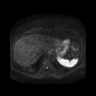
\includegraphics[width=.95\linewidth]{img_hyperopt/Abdomen_785}
        \end{subfigure}%
        \begin{subfigure}[b]{0.25\textwidth}
                \centering
                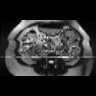
\includegraphics[width=.95\linewidth]{img_hyperopt/Abdomen_1050}
        \end{subfigure}%
        \begin{subfigure}[b]{0.25\textwidth}
                \centering
                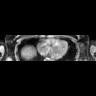
\includegraphics[width=.95\linewidth]{img_hyperopt/Abdomen_5115}
        \end{subfigure}%
        \begin{subfigure}[b]{0.25\textwidth}
                \centering
                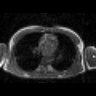
\includegraphics[width=.95\linewidth]{img_hyperopt/Chest_6810}
        \end{subfigure}
        
        \vspace*{2mm}
        
        \begin{subfigure}[b]{0.25\textwidth}
                \centering
                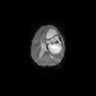
\includegraphics[width=.95\linewidth]{img_hyperopt/Head_13330}
        \end{subfigure}%
        \begin{subfigure}[b]{0.25\textwidth}
                \centering
                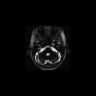
\includegraphics[width=.95\linewidth]{img_hyperopt/Head_14031}
        \end{subfigure}%
        \begin{subfigure}[b]{0.25\textwidth}
                \centering
                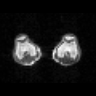
\includegraphics[width=.95\linewidth]{img_hyperopt/Legs_13170}
        \end{subfigure}%
        \begin{subfigure}[b]{0.25\textwidth}
                \centering
                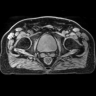
\includegraphics[width=.95\linewidth]{img_hyperopt/Pelvis_23016}
        \end{subfigure}
        \caption{Images from the MR dataset showing the variety of classes and protocols.}
        \label{fig:dataset}
\end{figure}

Given an MRI volume we would like to know which anatomical regions are contained in it and their position in the volume. Since MRI data are acquired in a slice by slice approach, we reduce the problem to a two dimensional classification task of axial slices (into head, chest, abdomen, pelvis, legs and spine).

\begin{table}[htb]
	\centering
	\begin{tabular}{ | l | c | r | }
		\hline
		Body Part & \# Volumes & \# Slices \\ \hline
		Head & 404 & 17011 \\
		Chest & 186 & 6897 \\
		Abdomen & 367 & 15486 \\
		Pelvis & 351 & 17962 \\
		Legs & 99 & 12868 \\
		Spine & 390 & 9790 \\
		\hline
	\end{tabular}
	\caption{Content of the MRI field-of-view dataset.}
	\label{table:dataset}
\end{table}

The dataset consists of MRI images coming from a variety of hospitals and machines across the world (such as the \textit{Centre Hospitalier Lyon-Sud, France} or \textit{ Johns Hopkins University, USA}). As a consequence the images are highly varied in terms of protocols (see Figure~\ref{fig:dataset}) as well as resolution, number of volumes per class and number of slices per volume. Table~\ref{table:dataset} sums up the content of our dataset.

The dataset is splitted into a training set for the optimization of the weights of the networks, a validation set for model selection (optimization of the hyper-parameters) and a test set for model evaluation (respectively $50 \%$, $25 \%$, $25 \%$ of the database). The separation is done volume-wise to take into account intra-subject slices correlations. Volumes containing multiple classes are split by anatomical regions and can end up in different sets. This raises the difficulty of the task since, in case of overfitting, predictions will be wrong at validation or testing phases.

%We also stratified classes across sets, giving us a proportion of slices per class close to the proportion of volumes per class.

Finally, each slice is subject to a unique step of preprocessing: it is resized to $128 \times 128$ pixels, a good trade-off between time constraints and quality of information.

Data augmentation is used and consists in generating 80 000 images per epoch. The augmentation is done by applying translations, shearing and rotations, zooming, and adding Gaussian noise.

%%%%%%%%%%%%%%%%%%%%%%%%%%%%%%%%%%
\subsection{Baseline results}

\begin{figure}[htb]
	\centering
	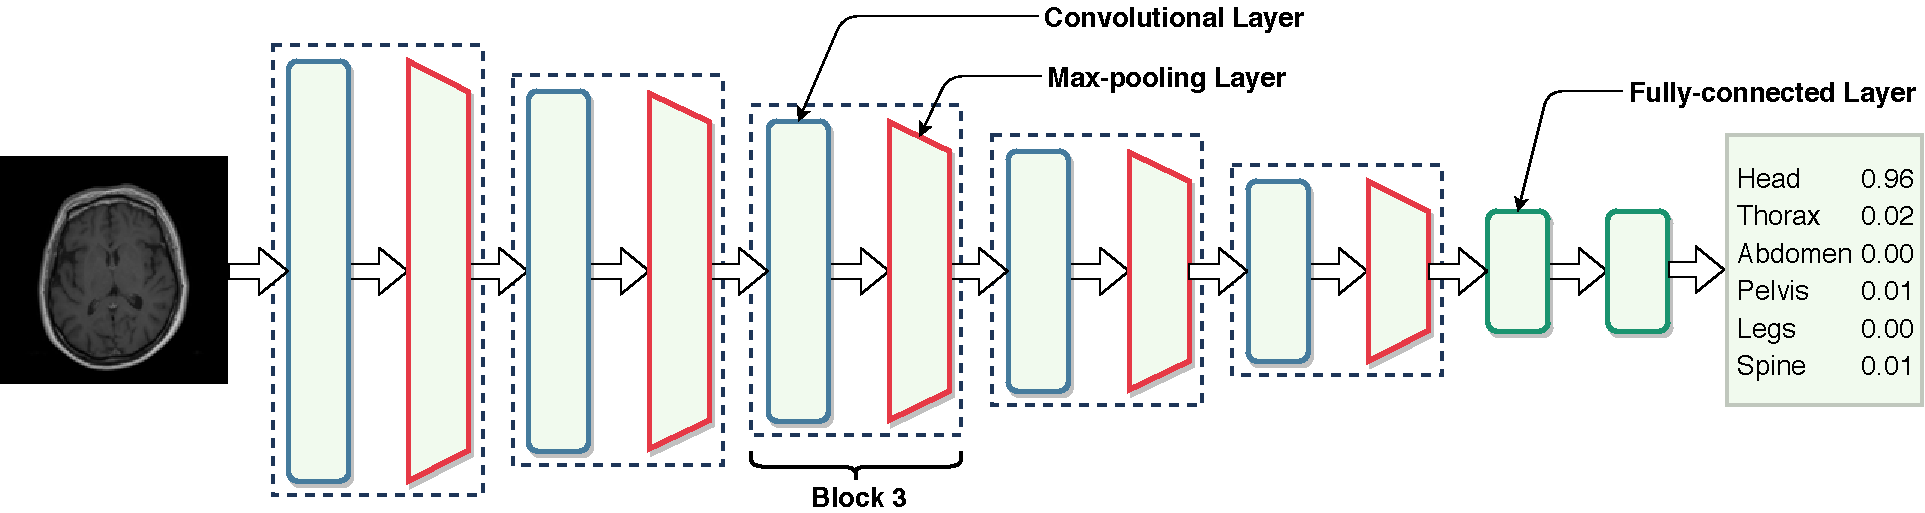
\includegraphics[width=\linewidth]{img_hyperopt/baseline.pdf}
	\caption{Baseline network used to solve the problem.}
	\label{fig:baseline}
\end{figure}

Starting from a standard VGG architecture (\textcite{simonyan2014}), we modified it manually until settling on the following model, shown in Figure~\ref{fig:baseline}: it is divided into 5 blocks, each comprising a convolution layer of 64 filters of size $3\times 3$, followed by a rectified linear unit (ReLu) and a max-pooling layer. The network ends with 2 fully-connected layers (respectively 4096 and 1024 units) interleaved with ReLU activations and terminated with a softmax decision layer. This network was trained by minimizing the categorical cross-entropy loss weighted by class frequency, using stochastic gradient descent (SGD) with a learning rate of $10^{-3}$, Nesterov momentum ($m = 0.9$) and decay ($d = 10^{-6}$) for 30 epochs.

\begin{table}
    \centering
    \newcommand\items{6}   %Number of classes
    \arrayrulecolor{white} %Table line colors
    \noindent\begin{tabular}{cc*{\items}{|E}|}
    \multicolumn{1}{c}{} &\multicolumn{1}{c}{} &\multicolumn{\items}{c}{\textbf{Predicted}} \\ \hhline{~*\items{|-}|}
    \multicolumn{1}{c}{} & 
    \multicolumn{1}{c}{} & 
    \multicolumn{1}{c}{\rot{Head}} & 
    \multicolumn{1}{c}{\rot{Chest}} & 
    \multicolumn{1}{c}{\rot{Abdomen}} &
    \multicolumn{1}{c}{\rot{Pelvis}} & 
    \multicolumn{1}{c}{\rot{Legs}} & 
    \multicolumn{1}{c}{\rot{Spine}} \\ \hhline{~*\items{|-}|}
    \multirow{\items}{*}{\rotatebox{90}{\textbf{Actual}}} 
    &Head  & 96 & 0 & 1 & 2 & 1 & 0   \\ \hhline{~*\items{|-}|}
    &Chest  & 1 & 57 & 13 & 28 & 1 & 0   \\ \hhline{~*\items{|-}|}
    &Abdomen  & 0 & 1 & 88 & 10 & 0 & 1   \\ \hhline{~*\items{|-}|}
    &Pelvis  & 1 & 0 & 9 & 81 & 8 & 1   \\ \hhline{~*\items{|-}|}
    &Legs  & 0 & 0 & 0 & 19 & 81 & 0   \\ \hhline{~*\items{|-}|}
    &Spine  & 0 & 1 & 3 & 2 & 0 & 94   \\ \hhline{~*\items{|-}|}
    \end{tabular}
    \caption{Confusion matrix for the baseline on the test set, in percent.}
	\label{table:conf_matrix_baseline}
\end{table}

We achieve a $14 \%$ error rate with most of the error focused on the chest. Examining the confusion matrix (Table~\ref{table:conf_matrix_baseline}), we note that the abdomen, pelvis and legs images have most of their errors located with anatomically adjacent regions. Further examinations of the misclassified images revealed they were for the most part located at the boundaries of their classes. These errors make sense as these boundaries are ill-defined and varies from one volume to the next. 

%%%%%%%%%%%%%%%%%%%%%%%%%%%%%%%%%%
\subsection{Hyper-parameter optimization}

\begin{figure}[htb]
	\centering
	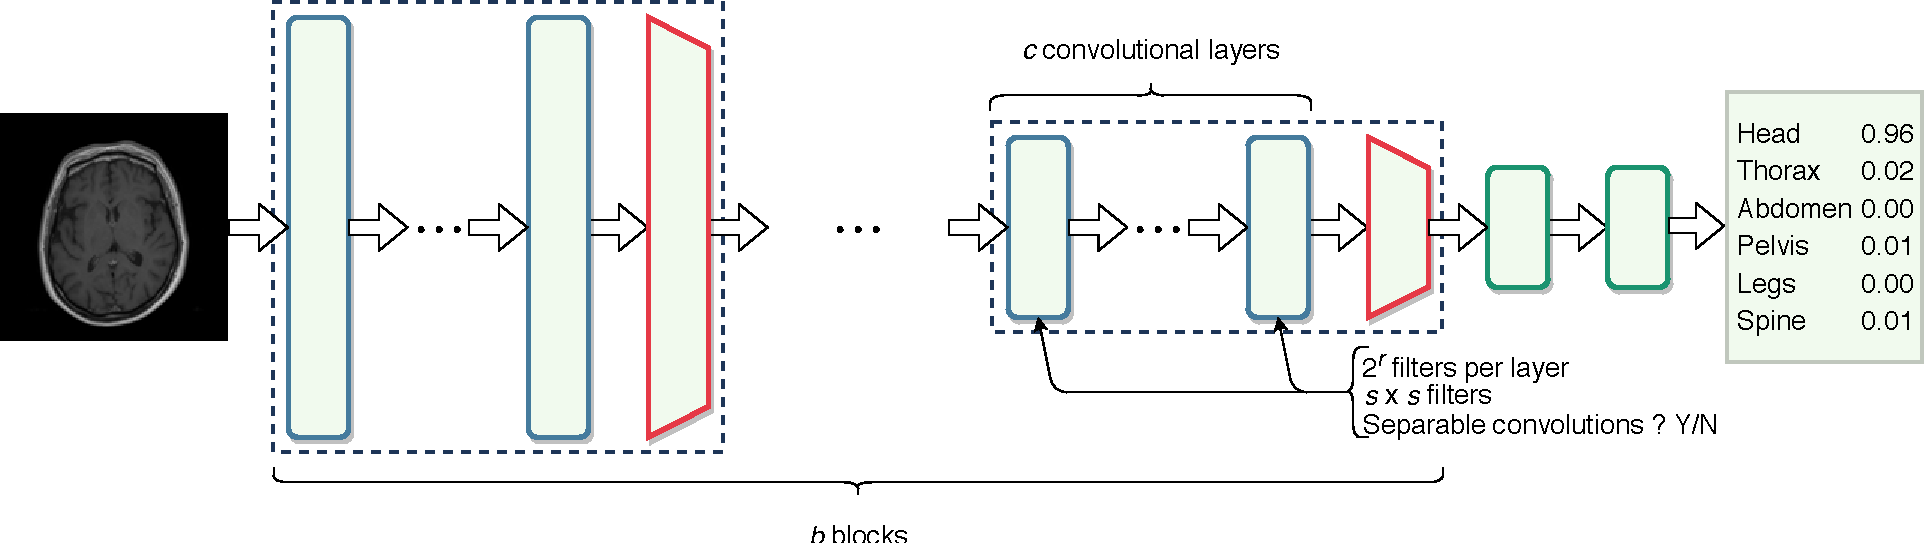
\includegraphics[width=\linewidth]{img_hyperopt/hyperspace.pdf}
	\caption{Variations on the baseline allowed in our search.}
	\label{fig:hyperspace}
\end{figure}

By relaxing some structural parts of our baseline architecture we define a large family of models. This hyper-parametric family has the following structure (see Figure~\ref{fig:hyperspace}): (1) $b$ convolution blocks, each including $c$ convolutional layers of $2^r$ filters of size $s \times s$ interleaved with ReLU activations and terminated by a max-pooling layer, (2) the fully-connected layers as in our baseline architecture, and (3) a final softmax decision layer. 

The last hyper-parameter is whether the convolutions are separable or not. Separable convolutions are two different convolutional layers using $1 \times 3$ filters then $3 \times 1$. This leads to a $33 \%$ reduction in the number of weights often without negative impact on the model performance.

Changes within this parametric space of models may drastically transform the optimization landscape, requiring to adjust the training setting accordingly (in our case: learning rate and batch size, all other settings remaining identical). 
These architecture hyper-parameters and training settings form the hyper-parameter space. The ranges of those hyper-parameters, detailed in Table~\ref{table:hyper}, were defined so as to fulfill memory (less than 12GB) and time constraints (training should last less than one day).

While many more hyper-parameters could have been considered, the ones we chose already define a search space of 34 300 models, well-above our capacity to fully explore. Those hyper-parameters were chosen as they were considered to have the highest impact on the performance by a mix of intuition and experience. A more systematic approach would likely yield better results, though at a greater computational cost.

\begin{table}
	\centering
	\arrayrulecolor{black}
	\begin{tabular}{ | l | c | r | }
		\hline
		Name & Range & Baseline \\ \hline
		Number of blocks & $b \in [1 ; 5]$ & $5$ \\
		Number of convolutional layers per block & $c \in [1 ; 5]$ & $1$ \\
		Number of filters per convolutional layer & $2^{r}, r \in [2, 8]$ & $64$ \\
		Size of the filters & $ s \in \{3 ; 5\}$ & $3$ \\
		Separable Convolutions & $e \in \{\text{Yes}, \text{No}\}$ & No \\
		Learning Rate & $10^{l}, l \in [-7 ; 0]$ & $0.001$ \\
		Batch Size & $2^{a}, a \in [2 ; 8]$ & 8 \\
		\hline
	\end{tabular}
	\caption{Description of the hyper-parameters, with their range and and the baseline value.}
	\label{table:hyper}
\end{table}

To explore this hyper-parameter space, we used Bayesian optimization, as described in Section~\ref{sec:bo}.\footnote{While the previous section suggests Hyperband is a better method, this work was done before Hyperband.} We chose the Expected Improvement as our acquisition function, and we used the loss on the validation set as the value the Gaussian process must predict. Every network was trained for 30 epochs, and we trained a total of 300 models. The first model picked by the Bayesian optimization is usually chosen randomly, here it made sense to start from the baseline as it was already trained.

\begin{figure}[htb]
	\centering
	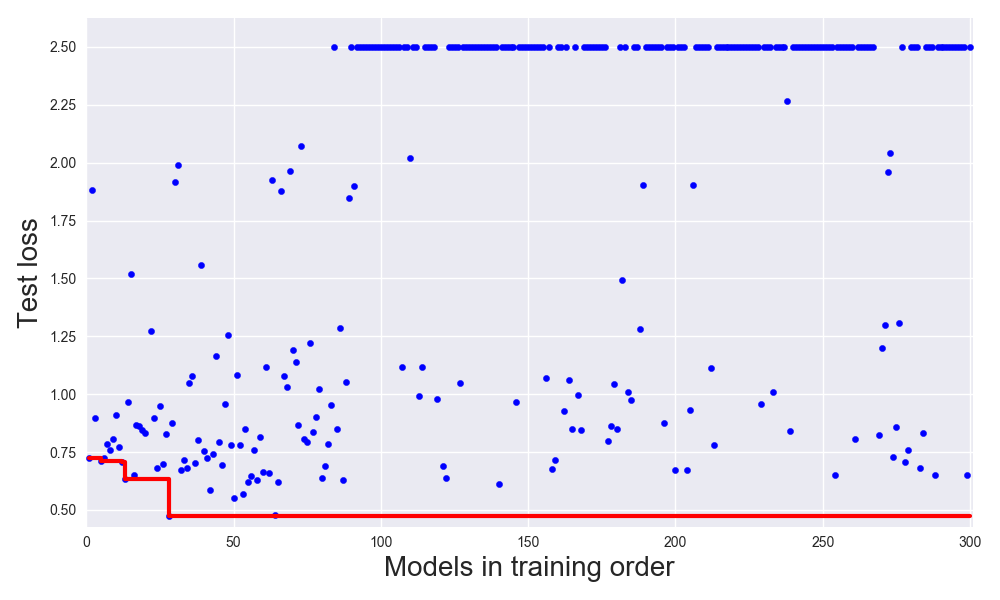
\includegraphics[width=\linewidth]{img_hyperopt/mrfov_bo_ei}
	\caption[Performance of the models in the order they were trained]{Performance of the models in the order they were trained. Each dot is a model. The red line represents the performance of the best model found until this point. The models with a loss of $2.5$ are models that could not be trained as they were too big.}
	\label{fig:mrfov_bo_ei}
\end{figure}

At the end, our optimization process yields a collection of models ranked by their performance. The quality of this assessment is naturally limited since the size of the validation set used in this respect cannot encompass the diversity of clinical reality. Cross-validation could be used to get a better estimator of the performance, but we cannot practically afford its costs. 

Figure~\ref{fig:mrfov_bo_ei} shows the performance of the models in the order they were trained. The baseline is quickly improved upon and the best model is found after 33 iterations. Another model with similar performance is found after 55 iterations. Starting at iteration 90, most of the chosen models are too big to fit in memory and therefore unable to train. While the fact that no previously chosen models were too memory intensive but suddenly most chosen models are may seem surprising, this can be explained for two reasons.

The first model of the process was our hand-crafted baseline, which had good performance. This likely allowed for a good initialization of the Gaussian process, and the following models explored the area around the baseline. As models explored further and further than the baseline, eventually one was chosen that was too big to fit in memory. This argument is speculation that should be confirmed by repeating the Bayesian optimization many times with a different initialization every time. Lack of resources prevented us from exploring this point further.

The second argument explains why most models became impossible to train as soon as the first of those was chosen. This is due to how we handled models impossible to train for memory limitations. We chose to simply remove such models from the search space. However the acquisition function still gives a high priority to this region of space and a surrounding model is chosen that is also likely to be too big. Since we remove those models on subsequent iterations, the acquisition function never learns to not go there.

An alternative way to handle un-trainable models would have been to choose an arbitrarily high loss for those models. This violates the smoothness assumption of the Gaussian process and would have affected strongly the prediction on nearby models, discouraging the acquisition function from choosing them. This would have also disqualified nearby models that fit in memory, which was our reason for not doing that in the first place. 

It is not clear which strategy is better. Choosing a high loss sacrifices some valid models, but saves time by testing less un-trainable models. On the other hand, an un-trainable model fails immediately at model creation, so the gain in time is minor. 
But independently of the chosen strategy, the fact that some combinations lead to model too big to fit in memory highlights a flaw in the design of the hyper-parameters space and the resulting networks architectures. The un-trainable models are models with a low number of blocks but a high number of filters per layer. With one block and 64 filters per layer, the feature maps of the last convolutional layer are of size $64 \times 48 \times 48$, meaning the following fully-connected layer have $64 \times 48 \times 48 \times 4096 = 603,979,776$ weights. Since each block ends with a max-pooling layer, the number of weights quickly becomes manageable with additional blocks. 

\begin{table}
    \centering
    \newcommand\items{6}   %Number of classes
    \arrayrulecolor{white} %Table line colors
    \noindent\begin{tabular}{cc*{\items}{|E}|}
    \multicolumn{1}{c}{} &\multicolumn{1}{c}{} &\multicolumn{\items}{c}{\textbf{Predicted}} \\ \hhline{~*\items{|-}|}
    \multicolumn{1}{c}{} & 
    \multicolumn{1}{c}{} & 
    \multicolumn{1}{c}{\rot{Head}} & 
    \multicolumn{1}{c}{\rot{Chest}} & 
    \multicolumn{1}{c}{\rot{Abdomen}} &
    \multicolumn{1}{c}{\rot{Pelvis}} & 
    \multicolumn{1}{c}{\rot{Legs}} & 
    \multicolumn{1}{c}{\rot{Spine}} \\ \hhline{~*\items{|-}|}
    \multirow{\items}{*}{\rotatebox{90}{\textbf{Actual}}} 
    &Head  & 94 & 0 & 1 & 1 & 2 & 0   \\ \hhline{~*\items{|-}|}
    &Chest  & 0 & 93 & 5 & 1 & 1 & 0   \\ \hhline{~*\items{|-}|}
    &Abdomen  & 0 & 2 & 85 & 10 & 2 & 1   \\ \hhline{~*\items{|-}|}
    &Pelvis  & 1 & 2 & 4 & 86 & 6 & 1   \\ \hhline{~*\items{|-}|}
    &Legs  & 0 & 4 & 1 & 19 & 76 & 0   \\ \hhline{~*\items{|-}|}
    &Spine  & 0 & 1 & 1 & 0 & 2 & 96   \\ \hhline{~*\items{|-}|}
    \end{tabular}
    \caption{Confusion matrix for the best model on the test set, in percent.}
	\label{table:conf_matrix_best}
\end{table}

The best model found with Bayesian optimization has an error rate of $10 \%$, an improvement of $4 \%$ over the baseline. Looking at the confusion matrix in Table~\ref{table:conf_matrix_best}, there is a significant improvement in the classification of chest, going from $57 \%$ accuracy in the baseline to $93 \%$ accuracy. The other classes have similar accuracy as the baseline. Most of the errors are abdomen and legs slices located at the boundaries of the pelvis.

Looking at the architectures of the two best models that have very similar error rates, it can be observed that the first one only deviates from the baseline by having two convolutional layers per block but only $32$ filters per convolutional layer and a higher batch size of $32$. The second model however is completely different. It has only 4 blocks with 3 convolutional layers per block, uses separable convolutions, with a smaller batch size of 4 and learning rate of $10^{-4}$.

The last important factor to consider is the total number of weights. The baseline model had $6,713,226$ weights, the best model had $5,468,778$, a $19 \%$ reduction. The second best model had $13,927,114$ weights due to using one less block than the other two models. Once again most of the weights are caused by the transition from the last convolutional layer to the first fully-connected layer. To improve these results the first step would be to better design this transition, either by controlling the number of max-pooling layers or by replacing the fully-connected layers with convolutional layers, as is typical of modern convolutional neural networks. 

\subsection{From probabilities to a decision}

\begin{figure}[htbp]
	\centering
	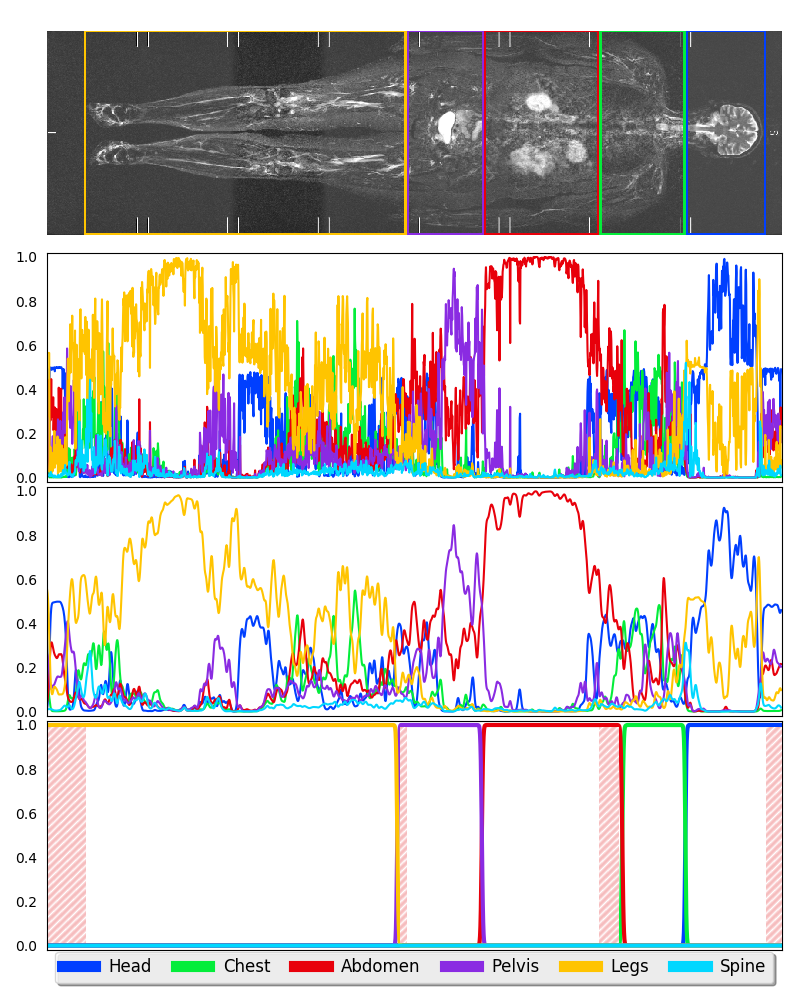
\includegraphics[width=\linewidth]{img_hyperopt/fullbody_error}
	\caption[Slice by slice prediction on a full body volume]{Slice by slice prediction on a full body volume. From top to bottom: (a) Image and ground truth. (b) Raw model prediction. (c) After smoothing. (d) Final prediction, after selecting the best transitions. Highlighted in red are the errors compared to the ground truth.}
	\label{fig:full_body}
\end{figure}

Even though we made the choice of processing the data at the slice level, the slices form volumes and we are interested in a decision at the volume level. The first question is: does the model classifies two successive slices similarly? This is expected since successive slices are anatomically close and have a similar structure. If the model gives very different predictions, this could be a sign that it relies on noise patterns instead of the anatomical structures.

To answer this question, we processed a full body volume by classifying each of its slices through our best model. 
%For each slice, the predicted class is the one with a probability higher than $0.7$, and if no class meets this criterion, then we do not choose any. 
As we can see in Figure~\ref{fig:full_body}, the network is able to identify all body parts, despite the slices being processed independently. Nevertheless the network tends to misclassify the boundaries between regions, notably legs/pelvis and pelvis/abdomen. It also mistakenly identifies the empty slices above the head as being pelvis with a high confidence. %This might be indicative of overfitting as those slices contain only noise. 
Interestingly, the straps used to hold the patient down, visible as the bands with high intensity on the extremities and low intensities on the body, trigger the network every time into the pelvis class. This is likely due to the rarity of those straps in the dataset.

But we are not interested in the mere probabilities, we want to take an actual decision. Therefore we need a decision scheme. A very simple one would be a threshold, say $0.7$, over which we consider the slice to be part of the class. However the predictions from the network are too noisy (see Figure~\ref{fig:full_body}-b), and this approach gives regions broken in multiple parts with messy boundaries.

A first step is to smooth the probabilities curves with a Gaussian filter, as illustrated in Figure~\ref{fig:full_body}-c. This makes the predictions easier to read, and we can see on this example that the predictions are correct almost everywhere except for the chest. Additionally, the pelvis is preceded and followed by the abdomen, which is of course impossible.

From this last observation, we note that our goal is to find contiguous anatomical regions, delimited by a starting slice $Z^m_i$ and an ending slice $Z^M_i$, where $i$ is the index of the region in anatomical order (legs - pelvis - abdomen - chest - head) and $Z$ is the slice number. Those boundaries must be such that 
%$\forall i \in [1; N], Z^m_i < Z^M_i$ (the ending slice is after the starting slice) and 
$\forall i \in [1; N], Z^m_{i+1} \ge Z^M_i$ (a region cannot start before the end of the previous region). The network outputs the probability of a slice to belong to a region $P_i \left( Z \right)$.

We translate these constraints on region boundaries and the fact that intuitively, the best region between two slices is the one that maximizes a region probability, through the following constrained linear program:
\begin{equation}
    \begin{array}{ll@{}ll}
    \text{minimize}  & - \displaystyle\sum\limits_{i=1}^{N} \int_{Z_i^m}^{Z_i^M} P_i(z) dz &\\
    \text{subject to}&  Z^m_{i+1} \ge Z^M_i,  &i=1 ,..., N
    \end{array}
    \label{eq:optimal_boundary}
\end{equation}

The Lagrangian is:
\begin{equation}
    \mathcal{L} \left( Z_i^m, Z_i^M, \lambda \right) = - \displaystyle\sum\limits_{i=1}^{N} \int_{Z_i^m}^{Z_i^M} P_i(z) dz
                                                        - \displaystyle\sum\limits_{i=1}^{N} \lambda_i \left( Z^m_{i+1} - Z_i^M \right)
\end{equation}
From the partial derivatives, we obtain:
\begin{align*}
    \frac{\partial \mathcal{L}}{\partial Z_i^m} &= P_i \left( Z_i^m \right) - \lambda_{i-1} \\
    \frac{\partial \mathcal{L}}{\partial Z_i^M} &= - P_i \left( Z_i^M \right) + \lambda_{i}
\end{align*}
Setting the derivatives at zero, the optimal boundary slices must verify:
\begin{equation}
    \lambda_i = P_i \left( Z_i^M \right) = P_{i+1} \left( Z_{i+1}^m \right)
\end{equation}
This result implies that the optimal boundary slices are the slices where adjacent regions intersect. For example, a slice where the probability of belonging to the pelvis is equal to the probability of belonging to the abdomen is a potential boundary slice, but an intersection slice between pelvis and head is not. We show an example of valid and invalid transitions slices in Figure~\ref{fig:valid_transitions}.

\begin{figure}[htbp]
	\centering
	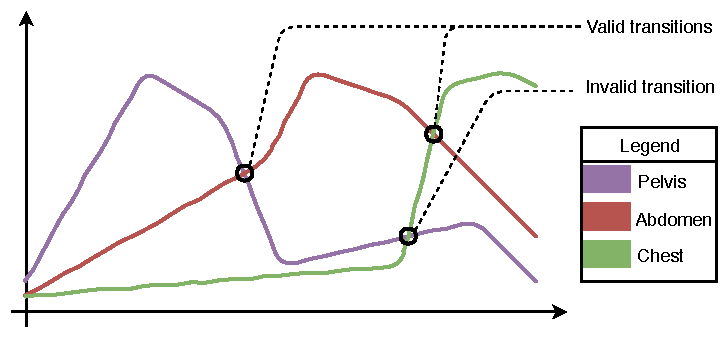
\includegraphics[width=\linewidth]{img_hyperopt/valid_transitions}
	\caption[Example of valid and invalid transitions]{Example of valid and invalid transitions. Pelvis/abdomen and abdomen/chest are valid as they are from adjacent classes, but chest/pelvis is invalid.}
	\label{fig:valid_transitions}
\end{figure}

To find the optimal boundary slices, we find all the valid intersection slices, construct all the valid sets of transitions and compute the function defined in Equation~\ref{eq:optimal_boundary}. The minimum is the optimal set of boundary slices. Following the example in Figure~\ref{fig:full_body}-d, the final prediction is wrong only at the extremities of the volume (our decision scheme forces to pick a class) and is in minor disagreement with the ground truth legs/pelvis boundary. The only error of consequence is the abdomen/chest boundary. Compared to the raw prediction which was wrong for the pelvis and chest, the improvement is clearly visible.

This scheme is robust because of its properties: each region is at most one contiguous block (it can also be not present), the regions are always in anatomical order and it allows for many misclassified slices. 

\subsection{Conclusion}

We have shown how to use Bayesian optimization to the concrete problem of MR FOV classification. The gain in performance between our handcrafted model and the best model clearly shows the value of automating the search of hyper-parameters, even with a limited budget.

The search was vulnerable to all the weaknesses of Bayesian optimization: the process was sequential (only one model trained at a time), we were limited in the hyper-parameters we could use (no conditional hyper-parameters) and the kernel was stationary. 
%As presented in Section~\ref{ssec:nosta}, work has been done on all those limitations and should be incorporated to improve the process. Other search methods could also be used, such as Hyperband (Section~\ref{sec:cap}). 

Another problem encountered is how to deal with models that cannot be trained (because they require too much memory for example). Not putting them in the training set will just let the search pick other similar models, but putting an arbitrarily high value is not ideal either as the Gaussian process will smoothly interpolate to that value, even though there is a discontinuity in that region (between the models that can and cannot be trained).

Regarding the final models, testing at the volume level has shown that the models are robust and can generalize. Still, the neural network was not enough to obtain smooth coherent predictions, and we presented a decision scheme to fix that.

Further work on this problem would involve improving the dataset by adding new volumes, new anatomical regions and defining stricter boundaries between regions. It could also be interesting to explore how to directly predict the boundaries of the regions using deep learning, instead of classifying each slice and using another method to obtain the regions. 

%%%%%%%%%%%%%%%%%%%%%%%%%%%%%%%%%%%%%%%%%%%%%%%%%%%%%%%%%%%%%%%%%%%%%%%%%%%%%%%%%%%%%%%%%%%%%%%
% \section{Conclusion}

% When to optimize and with which method ?
